\addcontentsline{toc}{section}{Abstract}
\section*{Abstract}
Past data collection efforts have led to the release of diverse trait databases in the public domain. Nevertheless, there is to date no database of terrestrial vertebrate species traits encompassing all four classes (birds, mammals, amphibians and reptiles).

Here, I compiled trait data information and range sizes from a variety of primary sources  across 5502 mammalian, 10334 reptilian, 11637 avian and 6904 amphibian species. Compiled traits related to species morphology (body mass), to life-history and behaviour (litter/clutch size, longevity, diel activity), to species habitat preferences (habitat breadth, natural habitat specialisation), and to species diet (trophic level; for mammals, birds and amphibians only, primary diet and diet breadth were also collected).

Before compiling the data, I extracted species accepted binomial names from the IUCN Red List and the Integrated Taxonomic Information System. I then harmonised taxonomy across primary sources. This procedure allowed to match dataset by species names more efficiently and enhanced the amount of trait information available. 

Trait data presented important taxonomic biases, with mammals and birds being significantly better sampled than herptiles. Trait information was also phylogenetically biased, particularly in herptiles, where entire clades were less well sampled than others. Finally, widespread species were more likely to have more traits sampled than narrow-ranged species.

I imputed missing trait values using random forest algorithms. Species phylogenetic relatedness was included as an additional predictor of trait values. Overall, imputations were robust, although imputations performed less well at predicting habitat related variables than other traits. 




\section{Introduction}
Planetary anthropogenic threats are reshaping patterns of species diversity \citep{ Spooner2018, Bohm2013, Schipper2008, Stuart2004}. Land-use change globally impacts local species richness (\cite{Newbold2015}). In turn, species losses can negatively affect ecosystem functioning (\cite{Hooper2005}, \cite{Hooper2012}). Understanding how increasing pressures will affect ecosystem functioning and the services ecosystems provide is vital to put into place efficient mitigation measures.
   
The earliest experiments investigating the effect of species richness on the stability of ecosystem processes were conducted in the late twentieth century \citep{Tilman1994, Naeem1994}. Hundreds of grassplot experiments have since then confirmed that higher diversity promotes higher primary productivity and increased ecosystem stability \citep{Tilman2014, Balvanera2006}. Intuitive mechanistic explanations of this phenomenon include increased niche complementary and resource partitioning, favouring more efficient resource use. Specifically, species properties (or traits) shape how species interact with their biological and physical environment. As such, traits are central to elucidate how species diversity links to ecosystem functions. 

Strictly, traits are defined as phenotypic characteristics measurable the level of an individual, with an effect on organismal fitness or performance \citep{McGill2006, Violle2007}. They can be physiological (e.g., metabolic rates), morphological (e.g., body mass), behavioural (e.g., activity time), phenological (e.g., anthesis); they can also relate to species life-history (e.g., longevity) or diet (e.g, trophic level).
Traits shape species fundamental and realised niches; for instance, physiological traits influence species thermal tolerances, participating in defining their geographical distributions \citep{Calosi2010, Khaliq2017}. Morphological attributes (e.g. body mass, eye position, etc.) participate in shaping the structure of food webs, and in determining the strength of inter- and intra-specific competition \citep{Gravel2016, Laigle2018}. As such, traits determine how species use and impact on their environment. Specifically, effect traits underpin species resource use and define organismal contributions to ecosystem functions. Response traits are those involved in determining species responses to environmental changes and can overlap with effect traits. This distinction between response and effect trait led to the development of a conceptual framework, the `response--effect' paradigm (\cite{Lavorel2002,Luck2012}; see Chapter 1), which aims to understand how traits shape species responses to environmental changes, and how these changes in turn affect ecosystem functioning. 

A looser, more flexible definition of trait is sometimes adopted. Some characteristics only measurable at the species level can be referred to as `ecological' traits. Examples of ecological traits, only measurable in relation to species occurrence, include habitat preferences (breadth or thermal/moisture preferences). In this Chapter, I use this more flexible definition of trait, and consider species `ecological' traits.

Trait-based approaches are increasingly used to understand processes underpinning species coexistence and biodiversity--ecosystem functioning relationships. Notably, they are widely employed in the context of the response--effect paradigm, and publications in this field have increased exponentially since the 2000s \citep{Hevia2017}. 

Nevertheless, studies investigating how species traits influence species responses to environmental changes, and how this may impact ecosystem functioning, are taxonomically and spatially biased\citep{Hevia2017}. Indeed, the metanalysis conducted by \citet{Hevia2017} showed that more than 75\% of such analysed studies considered plants or invertebrates. Moreover, about 60\% of the studies were conducted at local scales, while more than 90\% were conducted at local or national scales. Consequently, our understanding of biodiversity--ecosystem functioning relationships at various spatial scales need to be refined \citep{Thompson2018, Isbell2018}. Although vertebrates are one of the most studied group overall \citep{Titley2017}, how environmental changes may affect their global contributions to ecosystem functions needs to be investigated further. 

Indeed, vertebrates play diverse and important ecosystem roles \citep{Sekercioglu2006,Hocking2014,Severtsov2013}. Through frugivory, they  participate in seed dispersion \citep{Wandrag2015, Mokany2014, McConkey2012}. They are significant pollinators in numerous ecosystems \citep{Ratto2018}. Vertebrate herbivores impact global plant diversity patterns through top-down regulation \citep{Lin2018, Zhang2018}. They also contribute in regulating animal populations through their predatory activity \citep{Paine2016, Luck2012, Letnic2012, Salo2010, Barber2010}. As scavengers, they participate in nutrient cycling and energy transfers \citep{Cunningham2018, Inger2016, Wilson2011}. Moreover, they are culturally important \citep{Hirons2016, Albert2018}, and a source of protein for many people \citep{Alves2018}.

Understanding how environmental changes may affect their ecological roles is important to predict future ecosystem functioning, and to put into place appropriate mitigation measures. The end-goals of my PhD thesis include elucidating how species traits influence their responses to land-use and climate change at global scales, and how changes in community composition may affect ecosystem functions.

Addressing these questions requires to use extensive trait data. Despite vertebrates having been the focus of much research, and despite the growing interest for trait-based approaches, there exists no comprehensive database of vertebrate ecological traits encompassing all classes. Consequently, collating trait data was a prerequisite for any further work. This constituted the aim of the current Chapter: here, I collected and imputed trait data across the four terrestrial vertebrate classes (mammals, birds, reptiles and amphibians).

In this Chapter, I present the methods I used to collect and impute trait values across terrestrial vertebrates. Thanks to past and recent efforts to release data in the public domain, at least four ecological trait databases are now freely accessible (Table \ref{datasources}; \citet{Cooke2019}). Other trait datasets have been released on on-line platforms alongside published articles (e.g. Global Assessment of Reptile Distribution initiative, http://www.gardinitiative.org/), or can be downloaded from online databases (IUCN Red List (https://www.iucnredlist.org/), BirdLife data zone (http://datazone.birdlife.org/home). 

Data collection was constrained by the amount of information available in the literature.  All  primary sources offered a variety of traits, of which only a few were selected. Trait selection was motivated by two main reasons: (1) traits should be of ecological interest and be related to response or effect processes; (2) trait values should be available for many species, across the four terrestrial vertebrate classes, allowing for cross-classes comparative analyses. Targeted traits related to species life-history, morphology, behaviour and feeding habits (body mass; longevity; litter/clutch size; diel activity; trophic level; diet) and to their habitat preferences (habitat breadth and specialisation). Reptilian diet was not readily available in primary data sources, and one exception was made as I extracted diet data for the other classes (hence, I included diet despite it not being readily available for reptiles; reptile diet could be completed in the future). Species mobility was hardly available across sources, and no common variable could describe species mobility across classes. Although species' abilities to move in their environment is key in understanding how species will respond to anthropogenic pressures \citep{Schloss2012, Barbet-Massin2012,Pearson2006}, this trait was not considered for the above reasons. In addition to ecological traits, I also compiled species range sizes. In this Chapter, I detail the methodology I employed to collate targeted traits and range sizes. I elaborate on some of the challenges met when compiling data across many species, such as inconsistency of taxonomy across sources, and problems posed by taxonomic inflation and synonymy.

Despite a wealth of information across primary sources, trait data was likely to be incomplete across terrestrial vertebrates. Many species were likely to present missing trait data for many traits; and taxonomic and geographical biases in the global trait knowledge were likely to exist \citep{Hortal2014, Gonzalez-Suarez2012}. The gap in global trait knowledge was termed the `Raunki{\ae}r shortfall' by \citet{Hortal2014}. Here, I assessed the Raunki{\ae}r shortfall for terrestrial vertebrates. I investigated whether trait data presented taxonomic, phylogenetic and spatial biases.  

After examining patterns in the gaps in trait data information, I imputed missing trait values. This Chapter finally details imputation methodology and examines imputation performance and robustness.

%In October 2018, Cooke et al released a comprehensive database of six mammalian and avian traits. They collated and imputed missing trait values for body mass, litter/clutch size, volancy, diel activity, primary diet and habitat breadth. As similar primary sources were used in both our data collection, I did not use their database to complement my sources. Moreover, the imputation methods they used to fill gaps in trait coverage differed from mine. I used this freely accessible compiled data as an opportunity to compare the results of both our data collection and imputation processes. Results of this comparison are available in the SI.


\section{Methods}

\subsection{Ecological trait data collection}

\subsubsection{Primary data sources.}
I collated ecological trait data for terrestrial vertebrates from the sources figuring in Table \ref{datasources}. Information was compiled for the following target traits: body mass, longevity, litter or clutch size, trophic level, diel activity, diet, and habitat preferences. I also compiled traits that were potentially correlated to either body mass or longevity, to be used as potential predictors in imputations of missing trait values \citep{Meiri2010,Christiansen1999,AnAge}. As such, body length information was compiled when available, as well as generation length or age at sexual maturity. Most notably, longevity was chosen over generation length or age at sexual maturity as it was the only common currency across classes reflecting generation turnover. In addition, species geographical range sizes were estimated from distribution data, extracted from the IUCN Red List of Threatened Species.

% Table of sources.
\begin{table}[h!]
\renewcommand{\baselinestretch}{1}
\renewcommand{\arraystretch}{1.5}
\begin{center}\fontsize{9}{11}\selectfont
\caption[Primary sources used for each compiled trait.]{\textbf{Primary sources used for each compiled trait.} Primary sources may contain more traits than shown here. \textbf{BM}: body mass; \textbf{BL}: body length; \textbf{L}: longevity or maximum longevity; \textbf{GL}: generation length; \textbf{LCS}: litter or clutch size; \textbf{TL}: trophic level; \textbf{Di}: diet; \textbf{DA}: diel activity; \textbf{RS}: range size; \textbf{H}: habitat data. Bolded abbreviations highlight target traits; other traits were added for potential correlations in further imputations. $^1$Unpublished compilation of data; $^2$ http://datazone.birdlife.org/home; $^3$ https://www.iucnredlist.org/resources/spatial-data-download; $^{4}$http://apiv3.iucnredlist.org/api/v3/docs$\#$general.} 
\label{datasources}
\begin{tabular}{|l|c|c|c|c|c|c|c|c|c|c|c|c|}
\hline
\multicolumn{1}{|c|}{\multirow{2}{*}{\textbf{Sources}}} & \multirow{2}{*}{\textbf{Taxa}} & \multicolumn{9}{c|}{\textbf{Traits}} & \multirow{2}{*}{\textbf{RS}} & \multirow{2}{*}{\textbf{H}} \\ \cline{3-11}
\multicolumn{1}{|c|}{} &  & \textbf{BM} & BL & \textbf{L} & MA & GL & \textbf{LCS} & \textbf{TL} & \textbf{Di} & \textbf{DA} &  &  \\ \hline
\cite{Oliveira2017} & \multirow{4}{*}{Amphibians} & \checkmark & \checkmark & \checkmark & \checkmark &  & \checkmark & \checkmark & \checkmark & \checkmark &  &  \\ \cline{1-1} \cline{3-13} 
\cite{Cooper2008} &  &  & \checkmark &  &  &  & \checkmark &  &  &  & \checkmark &  \\ \cline{1-1} \cline{3-13} 
`Senior' dataset$^1$ &  &  & \checkmark &  &  &  &  &  &  &  &  &  \\ \cline{1-1} \cline{3-13} 
\cite{Sodhi2008} &  &  & \checkmark &  &  &  &  &  &  &  & \checkmark &  \\ \hline
\cite{Wilman2014} & \multirow{2}{*}{Birds} & \checkmark &  &  &  &  &  &  & \checkmark & \checkmark &  &  \\ \cline{1-1} \cline{3-13} 
BirdLife data zone$^2$ &  & \checkmark &  &  &  & \checkmark &  &  &  &  &  &  \\ \hline
\cite{Jones2009} & \multirow{5}{*}{Mammals} & \checkmark & \checkmark & \checkmark & \checkmark &  & \checkmark &  &  & \checkmark &  &  \\ \cline{1-1} \cline{3-13} 
\cite{Kissling2014} &  &  &  &  &  &  &  & \checkmark &  &  &  &  \\ \cline{1-1} \cline{3-13} 
\cite{Gainsbury2018} &  &  &  &  &  &  &  & \checkmark &  &  &  &  \\ \cline{1-1} \cline{3-13} 
\cite{Wilman2014} &  & \checkmark &  &  &  &  &  &  & \checkmark & \checkmark &  &  \\ \cline{1-1} \cline{3-13} 
\cite{Pacifici2013} &  & \checkmark &  & \checkmark & \checkmark & \checkmark &  &  &  &  &  &  \\ \hline
\cite{Scharf2015} & \multirow{8}{*}{Reptiles} & \checkmark &  & \checkmark & \checkmark &  & \checkmark & \checkmark &  & \checkmark &  &  \\ \cline{1-1} \cline{3-13} 
%Meiri &  &  &  &  &  &  &  & \checkmark &  & \checkmark &  &  \\ \cline{1-1} \cline{3-13} 
\cite{Vidan2017} &  &  &  &  &  &  &  &  &  & \checkmark &  &  \\ \cline{1-1} \cline{3-13} 
\cite{Stark2018} &  & \checkmark &  & \checkmark &  &  & \checkmark &  &  & \checkmark &  &  \\ \cline{1-1} \cline{3-13} 
\cite{Schwarz2017} &  &  &  &  &  &  & \checkmark &  &  &  &  &  \\ \cline{1-1} \cline{3-13} 
\cite{Novosolov2017} &  & \checkmark &  &  &  &  &  & \checkmark &  &  & \checkmark &  \\ \cline{1-1} \cline{3-13} 
\cite{Novosolov2013} &  &  &  &  &  &  & \checkmark &  &  &  &  &  \\ \cline{1-1} \cline{3-13} 
\cite{Slavenko2016} &  & \checkmark &  &  &  &  &  &  &  &  &  &  \\ \hline
\cite{Myhrvold2015} & Amniotes & \checkmark & \checkmark & \checkmark & \checkmark &  & \checkmark &  &  &  &  &  \\ \hline
IUCN Red List$^{3,4}$ & Vertebrates &  &  &  &  &  &  &  &  &  & \checkmark & \checkmark \\ \hline
\end{tabular}
\end{center}
\end{table}

\subsubsection{Compilation methods.}

\paragraph{Continuous traits.}
All continuous traits were averaged within species when different sources provided estimates. Longevity and maximum longevity were assumed to provide the same information and were averaged within species. Due to the scale of the data compilation, as well as the data availability, no measure of intra-specific variability was compiled. Estimates were provided as a single measure for each species, despite intra-specific variation being increasingly recognised as having important effects on ecological systems \citep{Bolnick2011,DesRoches2018, Siefert2015}.

\paragraph{Categorical traits.}
\subparagraph{Activity time.}
Species were described as being either nocturnal or non-nocturnal. Despite a higher resolution of activity time information in some of the primary sources (e.g. species being described as cathemeral, crepuscular or strictly diurnal), I adopted the classification of the primary source with the lowest resolution, in order to have consistent information across classes.
As such, all species defined as diurnal, cathemeral or crepuscular were classified as non-nocturnal, as opposed to species classified as strictly nocturnal.
\subparagraph{Primary diet.}
Here, I aimed to describe species primary diet, that is, if possible, the diet based on food items representing more than 50\% of species consumption. For mammals and birds, diet information was compiled from the EltonTraits database (\cite{Wilman2014}). Primary diet was available in the avian dataset in \citet{Wilman2014} and grouped into five categories: (1) plant or seed consumers; (2) fruit or nectar consumers; (3) vertebrate consumers, including fish and carrion; (4) invertebrate consumers; and (5) omnivores. I used these categories for other classes.

Primary diet was not available for mammals. Instead, mammal diet was described as the percent use of different food items. I pooled these items together into the same five primary diet categories as for the avian dataset. Below and in Table \ref{table_diet}, I explain the procedure I followed to define the primary diet for mammals.

The food items that were described for mammals in \citet{Wilman2014} were: invertebrates; vertebrates (either ectotherms, endotherms, fishes, carrion or other); fruit; nectar; seeds; and other plant material. I started by summing the percent uses of different vertebrate food items to define an overall percent use of vertebrates. I then used the percent use in each category to define the primary diet, as detailed below:
\begin{itemize}
\item If all food items had a percent use strictly below 50\% percent, the species was classified as omnivore.
\item If one food item only had a percent use above or equal to 50\%, the primary diet was defined with the corresponding item.
\item Finally, if two food items had a percent use equal to 50\%, the diet was defined depending on the combination of food items. Species with equal use of fruit and nectar were described as fruit and nectar consumers.  Species with equal use of plants and seeds were described as plant and seed consumers. Species with any other combination of food items were considered omnivores. 
\end{itemize}


For amphibians, diet information was extracted from AmphiBIO (\cite{Oliveira2017}). Diet information was available as binary variables for diverse food items (leaves, flowers, seeds, fruit, arthropods and vertebrates). Percent use was not recorded, so all items listed for a given species were considered to form species primary diet. I pooled amphibian diet into the five diet categories described above (procedure explained in Table \ref{table_diet}).

\begin{table}[h!]
\renewcommand{\baselinestretch}{1}
\renewcommand{\arraystretch}{1.5}
\begin{center}\fontsize{9}{11}\selectfont
\caption[Definition of primary diet based on consumption of food items for mammals and amphibians.]{\textbf{Definition of primary diet based on consumption of food items for mammals and amphibians.} \textbf{PU:} percent use. The table shows how primary diet was determined for mammals and amphibians. For mammals, a percent use was available. On the other hand, for amphibians, food items were either consumed or not. When only one item was known to be consumed by a species (with PU\textgreater{}50\% for mammals), the primary diet was entirely defined by the consumed item. When several items were consumed, primary diet was defined depending on the combination of items. There were particular cases for mammals: when all items had PUs\textless{}50\%, the corresponding species were considered to be omnivores.} 
\label{table_diet}
\begin{tabular}{|l|l|l|l|l|}
\hline
\multicolumn{1}{|c|}{\multirow{3}{*}{\textbf{\begin{tabular}[c]{@{}c@{}}Food items for\\ mammals\\ (percent uses)\end{tabular}}}} & \multicolumn{1}{c|}{\multirow{3}{*}{\textbf{\begin{tabular}[c]{@{}c@{}}Food items for\\ amphibians\\ (binary)\end{tabular}}}} & \multicolumn{3}{c|}{\textbf{Definition of primary diet}}                                                                                                                                                                                                                                                                                                                                                                \\ \cline{3-5} 
\multicolumn{1}{|c|}{}                                                                                                            & \multicolumn{1}{c|}{}                                                                                                                 & \multicolumn{1}{c|}{\multirow{2}{*}{\textbf{\begin{tabular}[c]{@{}c@{}}One item consumed:\\ Mammals: PU\textgreater{}50\%; \\ Amphibians: any item\end{tabular}}}} & \multicolumn{2}{c|}{\textbf{Several items consumed}}                                                                                                                                                                                           \\ \cline{4-5} 
\multicolumn{1}{|c|}{}                                                                                                            & \multicolumn{1}{c|}{}                                                                                                                 & \multicolumn{1}{c|}{}                                                                                                                                                  & \multicolumn{1}{c|}{\textbf{\begin{tabular}[c]{@{}c@{}}Mammals: \\ PU\textless{}50\%\end{tabular}}} & \multicolumn{1}{c|}{\textbf{\begin{tabular}[c]{@{}c@{}}Mammals: 2 items (PU=50\%)\\ Amphibians: any number.\end{tabular}}} \\ \hline
Vertebrates                                                                                                                       & Vertebrates                                                                                                                           & Vertebrate                                                                                                                                                    & Omnivore                                                                                             & + any others: Omnivore                                                                                                                \\ \hline
Invertebrates                                                                                                                     & Arthropods                                                                                                                            & Invertebrate                                                                                                                                                  & Omnivore                                                                                             & + any others: Omnivore                                                                                                                \\ \hline
Fruit                                                                                                                             & Fruit                                                                                                                                 & Fruit/nectar                                                                                                                                                  & Omnivore                                                                                             & \begin{tabular}[c]{@{}l@{}}+ nectar/flowers: Fruit/nectar\\ + any others: Omnivore\end{tabular}                           \\ \hline
Nectar                                                                                                                            & Flowers                                                                                                                               & Fruit/nectar                                                                                                                                                  & Omnivore                                                                                             & \begin{tabular}[c]{@{}l@{}}+ Fruit/nectar\\+ any others: Omnivore\end{tabular}                                    \\ \hline
Seeds                                                                                                                             & Seeds                                                                                                                                 & Plant/seed                                                                                                                                                    & Omnivore                                                                                             & \begin{tabular}[c]{@{}l@{}}+ OPM/leaves: Plant/seed\\+ any others: Omnivore\end{tabular}                                 \\ \hline
\begin{tabular}[c]{@{}l@{}}Other plant\\ material (OPM)\end{tabular}                                                              & Leaves                                                                                                                                & Plant/seed                                                                                                                                                    & Omnivore                                                                                             & \begin{tabular}[c]{@{}l@{}}+ seeds: Plant/seed\\+ any others: Omnivore\end{tabular}                                      \\ \hline
\end{tabular}
\end{center}
\end{table}

\subparagraph{Diet breadth.}
Diet breadth was defined as the number of primary food items recorded for a species.


\subparagraph{Trophic level.} Species were described as omnivores, carnivores or herbivores. For amphibians and birds, trophic levels were partly inferred from the primary diet (where primary diet information was available where trophic level was not). An omnivore primary diet directly translated into the omnivore category of trophic level. Vertebrate and invertebrate consumers were classified as carnivores. Fruit or nectar consumers and plant or seed consumers were classified as herbivores.

\subparagraph{Habitat preferences.}
Species habitat preferences were compiled from habitat data files downloaded from the IUCN Red List. In the files, all habitats known to be used by a given species were recorded. Overall, there were 96 habitat types. In addition, the suitability of each habitat was recorded (either marginal, suitable or unknown suitability), as well as the importance of the habitat for the species (either major, not major or unknown importance).

I pooled the 96 habitat types into 13 broader habitat categories (Forest, Savannah, Grassland, Shrubland, Wetland, Rocky areas, Caves and subterranean, Desert, Marine, Marine intertidal or coastal/supratidal, Artificial, Introduced vegetation and Other/Unknown). Whether a species was known to occur in these habitats was then encoded as a binary variable. I derived the two following variables from these files.

\textbf{Habitat breadth.}
I calculated habitat breadth as the number of habitats a species was known to use. I assigned weights to each habitat depending on the recorded suitability and importance of the habitat. As such, habitat breadth was calculated as $\sum_{i} w_{i} \cdot H_{i}$, where $H_{i}$ is the value of the binary variable for the $i^{th}$ habitat type (1: the species occurs in the $i^{th}$ habitat type; 0: the species is not known to occur in the $i^{th}$ habitat type); and $w_{i}$ is the weight assigned given the suitability$\times$importance combination (Table \ref{table_weights}). Outcomes were not very sensitive to the presence of weights (see SI for a comparison of the distributions of habitat breadths for the weighted sum versus the non-weighted sum -- where all $w_{i}$ equal 1). 

\begin{table}[h!]
\renewcommand{\baselinestretch}{1}
\renewcommand{\arraystretch}{1.5}
\begin{center}\fontsize{9}{11}\selectfont
\caption[Weights used in the calculation of habitat breadth]{\textbf{Weights used in the calculation of habitat breadth.} Habitat breadth was calculated as the weighted sum of the number of habitats used by a species. Weights were assigned to each habitat given its importance and its suitability. The rationale was that habitats that were not of major importance, or that were marginally suitable, should account for less in the sum. To be conservative, I assigned a weight of 1 to suitable/unknown habitats of unknown importance.} 
\label{table_weights}
\begin{tabular}{|l|c|c|c|}
\hline
\multicolumn{1}{|c|}{\multirow{2}{*}{\textbf{Suitability}}} & \multicolumn{3}{c|}{\textbf{Major importance}} \\ \cline{2-4} 
\multicolumn{1}{|c|}{}                             & \textbf{Yes}       & \textbf{No}        & \textbf{Unknown}       \\ \hline
\textbf{Suitable}                                           & 1         & 0.5       & 1             \\ \hline
\textbf{Marginal}                                           & 0.3       & 0.3       & 0.3           \\ \hline
\textbf{Unknown}                                            & 1         & 0.3       & 1             \\ \hline
\end{tabular}
\end{center}
\end{table}

\textbf{Degree of habitat specialisation.} Here, I classified species as being either natural habitat specialists or habitat generalists. If any artificial habitat was recorded to be suitable, species were reported to be generalists; else, species were natural habitat specialists. More details on habitat preferences compilation are provided in the SI. 

\subsection{Phylogenetic information}
I obtained phylogenetic trees for birds, amphibians, mammals and squamates from \citet{Hedges2015}. \citet{Hedges2015} built a time-calibrated phylogenetic tree representing more than 50,000 species, using meta-analytic methods: results from 2274 phylogenetics and molecular evolution studies were assembled to build a `Super Time' tree of life. Tree subsets for diverse clades are available at http://www.biodiversitycenter.org/ttol (downloaded 06/07/2018). The trees for vertebrate species were all ultrametric and fully resolved, except for the amphibian tree which presented polytomies (resolved later with multi2di, ape package: \citep{ape}). All trees contained a few branches of length 0 (193 branches for mammals, 136 for amphibians, 189 for birds and 284 for reptiles; these branches were modified later). Using trees that were built using molecular data, and not life-history traits, allows to avoid circularity in further imputations of missing trait values.


\subsection{Tackling taxonomic synonymy}
Across the different primary sources, similar species could appear under different binomial names. This was a problem when matching datasets by species. It was also problem when matching species to the PREDICTS database. Moreover, it is possible that within a primary source, a given species was appearing under two or more different names. As such, taxonomic synonymy created `pseudoreplicates' of the same species, overall falsely increasing the total number of species and artificially inflating the amount of missing trait values. Taxonomic synonymy was hence a major issue; due to the large number of species across datasets, extensive manual checks could not be applied. The presence of typos in species names had the same effect as synonymy, erroneously duplicating species. I attempted to correct for taxonomy first by correcting for typos, and second by identifying species which were entered under a synonymic name and replacing these with the accepted name. To this end, I developed an automated procedure, complemented with a few manual entries. Obvious cases where vernacular names had been entered in the place of binomial names were also treated manually; that was the case for 44 PREDICTS species (when possible, I best assigned binomial names to species common names; unidentifiable species were left empty and assigned to a genus (5 species)).

\subsubsection{Automated procedure and outputs.}
\paragraph{Extracting names from the IUCN Red List and the Integrated Taxonomic Information System (ITIS).}
The objectives of the automated procedure were to (1) extract species synonymic binomial names from the IUCN Red List or from the ITIS (rredlist and taxize R packages: \citet{rredlist}, \citet{Chamberlain2013}); and (2) identify the status of each name (accepted or not accepted). I started by generating a list of all names figuring across datasets (primary sources, phylogenies and PREDICTS). These `original' names were corrected for typos (using gnr$\textunderscore$resolve function, taxize package). Then, the IUCN Red List was queried and synonyms were stored when possible, as well as the status of each synonym. When species were not found in the IUCN Red List, information was extracted from the ITIS. When species were not found in the ITIS either, corrected names (original names corrected for typos) were assumed to be accepted. Family and order information was extracted using the same procedure and some entries were completed using the Global Biodiversity Information Facility taxonomic backbone (GBIF, https://www.gbif.org/tools/species-lookup).\\
\textbf{NB:} for species entered with the forms \textit{Genus cf.}, \textit{Genus aff.} or \textit{Genus spp.}, the accepted binomial name was left empty.

\paragraph{Outputs.} I generated a dataset containing records of all names (for 14124, 8743, 6090, and 11183 binomial names found across datasets for birds, amphibians, mammals and reptiles respectively, including species names as they appeared in phylogenetic trees). For each name, the identified accepted name and all other synonyms were stored when possible, as well as additional taxonomic information (order, family, genus). When queries did not succeed, species accepted names were assumed to be the original names found in the datasets (corrected for typos).

\paragraph{Harmonising taxonomy in trait datasets.}
Taxonomy across datasets was finally homogenised by replacing synonyms with their accepted scientific names. As a consequence, the total number of identified unique species decreased (Figure \ref{taxcor}). The species presenting the highest number of synonyms was the East African mole rat (\textit{Tachyoryctes splendens}), which was figuring under 12 names across primary sources (Figure \ref{taxcor}B), highlighting the need for normalising taxonomy across sources.

% figure: distribution of names and differences in species number
\vspace{0.5cm}
\begin{figure}[h!]
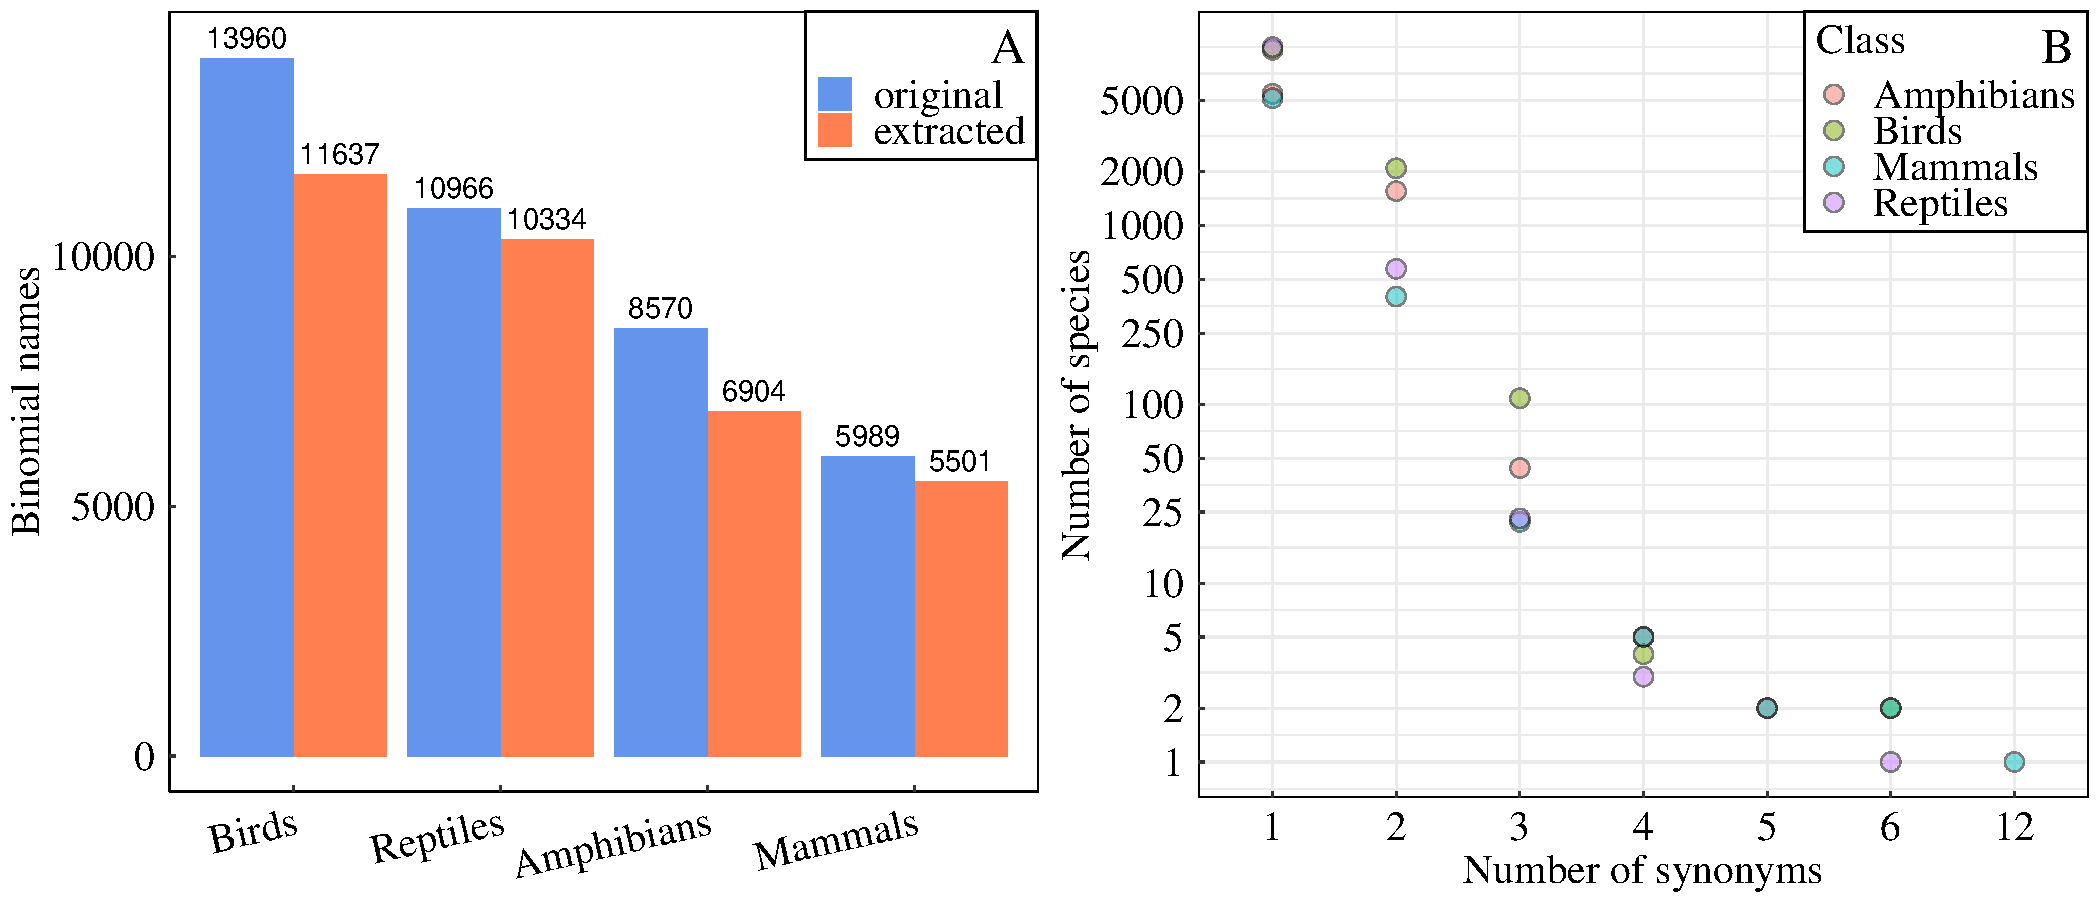
\includegraphics[scale=0.45]{figures/chapter2/Taxonomic_corrections/tax_corrections}
\caption[Difference in species number due to taxonomic correction (A) and distribution of number of synonyms across datasets (B)]{\textbf{Difference in species number due to taxonomic correction (A) and distribution of number of synonyms across datasets (B).} \textbf{(A)} shows the number of species across all primary sources (trait datasets and PREDICTS, excluding phylogenies), before and after correcting for taxonomy. Replacing identified synonyms by the extracted accepted name reduced the number of species in all classes, with the largest reduction for birds. \textbf{(B)} shows the distribution of the number of synonymic names. In all four classes, more than 5,000 species were known under one name only. Nevertheless, a large amount of species had two identified synonyms (range: 400 species for mammals - 2086 for birds). The most replicated species was the East African mole rat \textit{Tachyoryctes splendens}, for which 12 synonyms were identified.}
\label{taxcor}
\end{figure}

%Decrease by 2,323 unique binomial names for birds. The diminution was of 632 unique identified species for reptiles, of 1,666 for amphibians and of 488 for mammals.

At this stage, not all species in PREDICTS matched a species in the trait datasets. Additional manual inputs were required to resolve taxonomic synonymy for these species. Verifying the presence of PREDICTS species in trait datasets was important for further analyses. Taxonomic synonymy was resolved manually for 91 PREDICTS species that did not match any species in the trait datasets; in that case, information was extracted from other diverse sources (such as the Reptile Database (http://www.reptile-database.org/); Avibase (https://avibase.bsc-eoc.org/avibase.jsp?lang=EN\&pg=home); AmphibiaWeb (https://amphibiaweb.org/); and additional manual checks using the IUCN Red List for mammals). After adding manual inputs to the synonym datasets, all PREDICTS species were represented in trait datasets. 

The need to apply additional manual inputs underlines the fact that the automated procedure was not perfect. The Red List and the ITIS were not comprehensive taxonomic sources, and for clades with high degrees of `pseudoreplication' in names, such as reptiles or amphibians, neither the Red List or the ITIS contained enough information. As I only applied manual checks for a subset of species in the PREDICTS database, taxonomic redundancy and taxonomic errors are likely to have persisted to a degree in the trait datasets. Moreover, certain species were entered using the format \textit{Genus subspecies} rather than \textit{Genus species}; for these, automated queries may have failed to identify the species.

% Extract of synonym dataset? in the SI


\subsubsection{Harmonising taxonomy in phylogenetic trees and increasing species phylogenetic representation.}

\paragraph{Taxonomic correction across tip labels.} 
Efforts to correct datasets for taxonomy created problems for a small proportion of species when dealing with phylogenies. The idea of the procedure described above was to replace two or more identified synonyms by a single accepted name, and then collapsing dataset rows together by names. I applied the same method on phylogenies, replacing synonyms by their identified accepted names in trees' tip labels. As expected, in some cases, the procedure ended up assigning the same accepted name to different phylogenetic tips. This was the case for 2.8\% of mammalian, 1.7\% of avian, 1.6\% of amphibian and  1.7\% of reptilian species, which then had multiple phylogenetic positions (most having two different positions, see SI). Because keeping several putative phylogenetic positions for a species was problematic in further analyses, I selected one tip to conserve and dropped other tips from the phylogenies (Figure \ref{chart_phylorep}). 

To briefly describe the procedure, if replicated tips were sister clades, the tip to conserve was chosen randomly among the replicates. Presumably, selecting one sister clade or another would have an identical effect in that case. Else, I retained the tip that bore the accepted name in the original tree (when possible). In all other cases, tips to drop were chosen randomly. Further details on how replicated tips were dropped are available in the SI (with one example for each case of Figure \ref{chart_phylorep}).

\begin{figure}[h!]
\centering
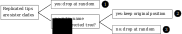
\includegraphics[scale=0.7]{figures/chapter2/chart_phylorep}
\caption[Procedure followed to drop replicated tips from phylogenies]{\textbf{Procedure followed to drop replicated tips from phylogenies.} Most replicated tip labels were replicated twice. The number in the boxes represent the number of occurrences across all four classes. \textbf{(1)} When replicated tips were sister clades, the tips to drop were chosen randomly, as it did not affect the `true' phylogenetic position of the species. \textbf{(2)} When replicated tips were not sister clades, I retained the tip that bore the accepted name in the uncorrected tree, when possible. \textbf{(3)} In a few cases, the accepted name did not appear in the original tree. This occurred when several tips bore names that were synonymic, but none of these were identified as being accepted. Those were problematic cases, and the tips to drop were chosen randomly. Nevertheless, occurrences of that third case were rare. See SI for more detailed information.}
\label{chart_phylorep}
\end{figure}

\begin{figure}[h!]
\centering
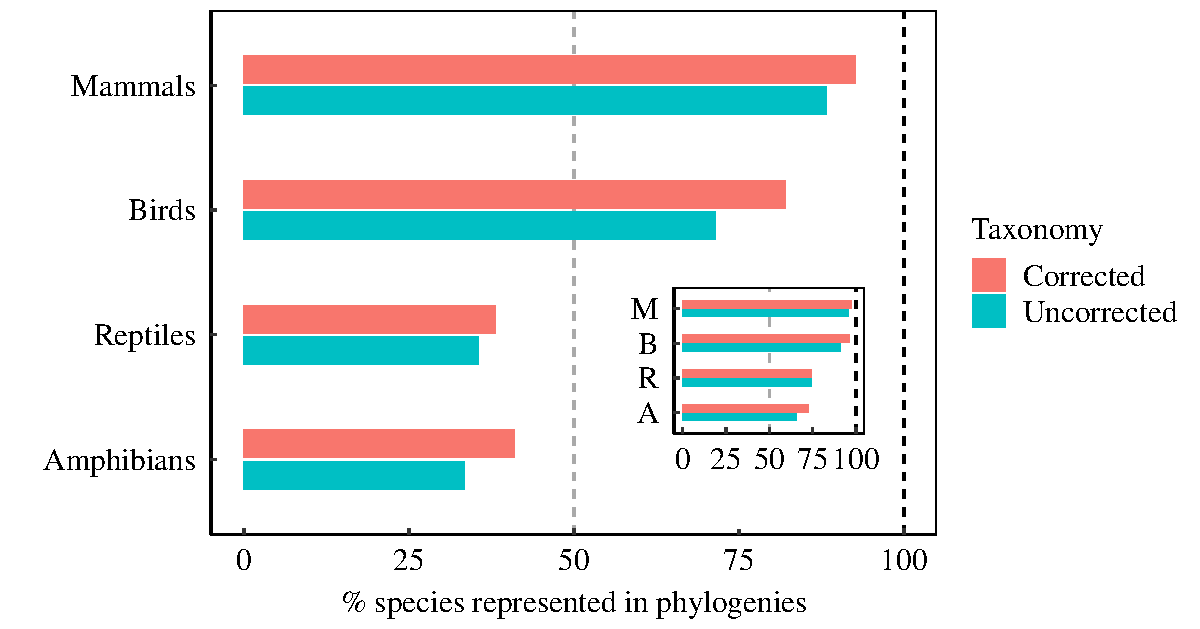
\includegraphics[scale=0.7]{figures/chapter2/Species_representation_phylo}
\caption[Percentage of species represented in the phylogenies, with and without taxonomic corrections]{\textbf{Percentage of species represented in the phylogenies, with and without taxonomic corrections.} The main plot shows the representation of species figuring in the trait datasets. Overall, taxonomic correction increased species representation in phylogenetic trees. Representation for mammals and birds was high (after taxonomic correction: 82\% of avian and 93\% of mammalian species had a phylogenetic position). On the other hand, reptiles and amphibians were poorly represented (after taxonomic correction: only 38\% of reptilian and 41\% of amphibian species were placed in phylogenetic trees). The inset barplot shows representation for species figuring in PREDICTS. For these, species presence in phylogenetic trees after correction was high across all classes, with a minimum representation of 76\% for amphibians.}
\label{species_rep_phylo}
\end{figure}

\paragraph{Correcting for taxonomy in the phylogenies: conclusions.}
Figure \ref{species_rep_phylo} shows the phylogenetic representation of species figuring in the trait datasets (as well as the representation of species figuring in PREDICTS, inset plot). Overall, correcting for taxonomy improved species representation in the trees. The representation of species figuring only in PREDICTS improved compared to the representation of all species (with a minimum representation of 76\% for PREDICTS amphibians after correcting the trees for taxonomy, inset plot in Figure \ref{species_rep_phylo}). Nevertheless, correcting phylogenetic tip labels generated replicates for a small number of tips, which then had to be dropped. 


\paragraph{Species attachments to phylogenetic trees.} Some species in the trait datasets were not represented in the phylogenies, even after taxonomic corrections (Figure \ref{species_rep_phylo}). Maximising the number of species represented in the phylogenies was important for further trait imputations. Indeed, if traits were evolutionary conserved, species phylogenetic position could be an important predictor of trait values. To maximise species representation, I attached non-represented species to the root of their genus, when possible, that is, when the genus was represented in the tree (phytools package: \citet{Revell2016}). Attaching species at the root of their genus created polytomies, which were resolved randomly (using multi2di in ape: \citet{ape},  and bifurcatr in PDcalc: \citet{PDcalc}). Resulting trees contained additional branches of length zero (which were modified later: see \textit{Measuring phylogenetic signal in categorical traits with $\delta$}). Such modifications of the phylogenetic trees could have altered the significance and the strength of trait phylogenetic signal. I further verified whether these alterations of the trees had impacted phylogenetic signal, by qualitatively comparing the strength and the significance of phylogenetic signal for each trait, estimated using both original trees and modified trees (see \textit{Assessing phylogenetic signal in traits}).

Finally, a large number of species were attached to their genus in the trees (Table \ref{random_attachments_phy}). For instance, only 38\% of the species figuring in the reptilian trait dataset were initially found in the squamate phylogeny. After attaching non-represented species, 91\% of the species were placed in the squamate phylogeny. 

\vspace{0.35cm}

\begin{table}[h!]
\renewcommand{\baselinestretch}{1}
\renewcommand{\arraystretch}{1.5}
\begin{center}\fontsize{9}{11}\selectfont
\caption[Species representation in phylogenetic trees (datasets corrected for taxonomy)]{\textbf{Species representation in phylogenetic trees (datasets corrected for taxonomy).} The number of species attached to the root of their genus ranged from 175 (mammals) to 5438 (reptiles). Finally, most species were represented in the phylogenies, whereas more than half reptilian and amphibian species initially had no known phylogenetic position.} 
\label{random_attachments_phy}
\begin{tabular}{|l|l|l|c|l}
\cline{1-4}
\multicolumn{1}{|c|}{\textbf{Class}} & \multicolumn{1}{c|}{\textbf{Not in tree}} & \multicolumn{1}{c|}{\textbf{Of which randomly attached}} & \textbf{No final representation in tree} &  \\ \cline{1-4}
Amphibians                  & 59\% (4040 of 6904)                           & 96\% (3883 of 4040)                     & \textbf{2.3\%}             &  \\ \cline{1-4}
Birds                       & 18\% (2085 of 11637)                          & 75\% (1574 of 2085)                    & \textbf{4.4\%}             &  \\ \cline{1-4}
Mammals                     & 7.4\% (407 of 5502)                           & 43\% (175 of 407)                       & \textbf{4.2\%}            &  \\ \cline{1-4}
Reptiles                    & 62\% (6391 of 10334)                          & 85\% (5438 of 6391)                    & \textbf{9.2\%}             &  \\ \cline{1-4}
\end{tabular}
\end{center}
\end{table}


\subsection{Investigating biases in the coverage and completeness of trait information across classes}

\subsubsection{Definition of trait coverage and trait completeness.}
\begin{itemize}
\item The coverage for a given trait was defined as the proportion of species for which an estimate was available. Trait coverage was calculated separately for each trait. \textbf{NB:} $1-$coverage then represents the proportion of missing values for a trait (here termed trait `missingness').
\item Trait completeness was defined for a given species as the proportion of traits that were estimated (number of non-missing trait values divided by total number of traits considered). Completeness was calculated over all predictor traits for each class (target traits and supplementary traits used in imputations). As such, the traits considered in each class were not necessarily the same (same set of target traits, but potentially diverse supplementary predictor traits).
\end{itemize}

\subsubsection{Taxonomic biases in coverage and completeness.}
Having normalised taxonomy and compiled trait data, I assessed trait coverage. I also calculated completeness across species in each class.

I tested whether taxonomic class impacted trait completeness using pairwise Kruskall-Wallis rank sum tests (the null hypothesis tested in each pair was that the distribution of completeness values were sampled from the same original distribution).
In addition, I investigated whether correcting for taxonomy had an effect on trait completeness using Wilcoxon rank sum tests. I tested whether the median trait completeness was significantly higher for datasets corrected for taxonomy, than for uncorrected datasets, in each class.
%In corrected datasets, species with 0\% completeness in predictor traits were filtered out.
% NB Wilcoxon used when two samples only; Kruskall-Wallis two or more samples.

\subsubsection{Phylogenetic biases in coverage and completeness.}
Whether values are missing at random phylogenetically is likely to impact imputation errors (but see \citet{Penone2014}). Further, I examined whether particular clades or parts of the phylogenies appeared to be under-sampled compared to other clades. To that end, I investigating whether missing trait values were distributed at random across the terminal branches of the phylogenies, using trait coverage and completeness. 

For each trait, I calculated the median missingness within each family. Within-family trait missingness was then plotted against phylogenetic trees built at the family level (using the function contMap of the phytools package: \citet{Revell2016}). Here, I generated one plot for each trait in each class.

I also calculated within-family median completeness. Similarly, within-family median completeness was plotted against phylogenetic trees built at the family level. One plot was generated for each class.

Families represented by few species might present higher percentages of missing values, reflecting family size rather than randomness in sampling. I added family trees representing the proportion of species in each family. 

\subsubsection{Spatial biases in completeness.} I finally investigated whether trait completeness was spatially biased. Specifically, I tested the hypothesis that bigger geographical range sizes were correlated with better trait completeness. To that end, I fitted a generalised linear model with a Poisson error distribution: trait completeness was treated as count data (number of sampled traits). Class was added as an explanatory factor, interacting with range size. The model was written as: Completeness $\sim$ log(RS) + Class + log(RS):Class, and I specified a Poisson error distribution. I examined whether the fit of the model was good using a chi-squared test on the residual deviance.

Additional analyses of spatial biases in trait sampling could be developed in the future.



\paragraph{Conclusion: imputing missing values to increase coverage.}
Trait coverage was highly variable across classes and traits (see Results). Trait coverage for species figuring in PREDICTS only improved compared to trait coverage for all species, particularly for reptiles and amphibians (see SI). Nevertheless, no trait reached 100\% coverage in any class. Moreover, within-class biases in availability of trait information appeared (see Results). Consequently, dropping missing-value species could skew trait distributions and generate biases in further analyses using the trait data. As such, rather than dropping missing-value species, I aimed to fill coverage gaps by imputing missing trait values. 

\subsection{Imputing missing trait values}
In order to achieve full coverage across classes, I imputed missing trait values. Diverse imputation methods have been developed and used in published articles \citep{Cooke2019, Molina-Venegas2018, Swenson2014}. \citet{Penone2014} assessed the performance of four different imputation approaches (K-nearest neighbour --kNN, \citet{Troyanskaya2001}--, multivariate imputation by chained equations --mice, \citet{mice}--, random forest algorithms as implemented in R by missForest \citep{Stekhoven2012, Stekhoven2016} and phylogenetic imputations implemented with PhyloPars \citep{Bruggeman2009}). Their study showed that the kNN approach resulted in significantly higher imputation error rates than the three other approaches. Both missForest and phylopars were the best methods when phylogenetic information was included. Nevertheless, phylopars was much slower than missForest, and could only handle continuous traits. missForest was faster and could deal with mixed type data. Without phylogenetic information, mice was found to be the best method, with fast imputations of mixed-type data. missForest was the best method when phylogenetic information was added. Of all these methods, missForest was the only one that did not make assumptions about data distribution (being a non-parametric approach), or that did not require a prior knowledge of some tuning parameters. As such, missForest appeared to be a robust option for missing data imputation. To further assess whether to use random forests rather than multivariate chained equations, I estimated the amount of phylogenetic signal in traits. Strong phylogenetic signal in traits would indicate than missForest could perform better than mice.

\subsubsection{Assessing phylogenetic signal in traits.}

\paragraph{Measuring phylogenetic signal in continuous traits with Pagel's $\lambda$.}
Phylogenetic signal is a measure of the tendency of closely related species to resemble each other more than less related species. Diverse statistics have been developed to estimate phylogenetic signal, most of them applying to continuous traits \citep{Munkemuller2012}. Here, I used Pagel's $\lambda$ \citep{Pagel1999} to assess the amount of phylogenetic signal in continuous traits. Pagel's $\lambda$ is a measure of the transformation of the internal branches of a phylogenetic tree required for a trait to have evolved under a pure Brownian motion model of evolution \citep{Munkemuller2012}. Under a Brownian motion model of evolution, changes in trait values happen at random along the branches and trait variance is proportional to evolutionary time.  When $\lambda=1$, the tree retains its internal structure and the branch lengths are not modified. This indicates that trait values are more similar in more closely related species (strong phylogenetic signal). When $\lambda=0$, the phylogeny becomes star-like, as all internal branches have a length of 0 (no phylogenetic signal).

Using Pagel's $\lambda$ (phylosig function, phytools package: \cite{Revell2016}), I assessed the strength of the phylogenetic signal. The phylosig function also allows to test for signal significance (comparing the estimated $\lambda$ to the null expectation of $\lambda$ with a log-likelihood ratio test). All traits were log-transformed to improve normality before estimating phylogenetic signal.

% In terms of branch length transformations, λ compresses internal branches while leaving the tip branches of the tree unaffected

\paragraph{Measuring phylogenetic signal in categorical traits with $\delta$ (\cite{Borges2018}).}
Very few methods have been developed to measure and test phylogenetic signal in categorical traits. \citet{Fritz2009} introduced the $D$-statistic; nevertheless, $D$ is based on a discretisation of categorical traits, which reduces them to binary variables. \citet{Borges2018} introduced a new statistic, called $\delta$, to measure phylogenetic signal in categorical traits. Their approach uses Bayesian inferences to reconstruct trait evolution, that is, to infer trait values in ancestral nodes of the phylogeny. The underlying idea is that the  better the phylogeny explains trait evolution, the lower the uncertainty in ancestral state inferences. As such, $\delta$ relies on the quantification of the uncertainty associated with the reconstruction of ancestral states. $\delta$ can take any positive number, with higher values indicating stronger signal. To test for the significance of the signal, the authors propose to compare the estimated value of $\delta$ with the null expectation  of $\delta$ (expectation given no phylogenetic signal), for instance by randomly attributing the trait vector to the phylogeny so as to generate a null distribution of $\delta$. 

I estimated phylogenetic signal in categorical traits with the $\delta$ statistic; implementation used the R code provided by \citet{Borges2018} (https://github.com/mrborges23/delta\textunderscore statistic). To test for the significance of the signal, I generated null distributions of $\delta$  for each trait by randomising trait vectors 50 times, and calculating $\delta$ for each randomised vector -- following the guidelines proposed by \citet{Borges2018}. I then calculated the median of simulated $\delta$ values as well as 95\% confidence intervals. I tested whether the null medians were significantly lower than the observed value of $\delta$ using one-sided Wilcoxon rank sum tests. I noted that the function developed by \citet{Borges2018} could not be implemented if phylogenetic trees contained branches of length 0. As both original and corrected phylogenies contained 0-length branches, I added a very small number to these ($10^{-10}$) to remedy to this issue and to test for phylogenetic signal. 

\paragraph{Significant phylogenetic signal in all traits.}
All traits showed significant phylogenetic signal (Table \ref{physignal} and SI for p-values of statistical tests), although the strength of the signal was variable across classes and traits. Overall, modifying the original phylogenies by correcting for taxonomy and by attaching species to the root of their genus did not, qualitatively, have a strong impact on the signal (Figures \ref{signalcontinuous} and \ref{signalcategorical}). In mammals and birds, phylogenetic signals remained similar. The bigger differences were observed for amphibian diet breadth (for continuous traits) and amphibian trophic level (for categorical traits), where adding species to the tree increased the strength of the signal.

Phylogenetic signal in categorical traits were all highly significant (Figure \ref{signalcategorical}; p-values for Wilcoxon signed rank test: see SI). The strength of the signal differed across classes and traits. The signal for habitat specialisation tended to be less strong (even though still highly significant). Diel activity, primary diet and trophic level showed strong phylogenetic signal across all classes. 

Most mammalian, avian and reptilian continuous traits had very strong phylogenetic signal ($\lambda \gtrsim 0.9$), except habitat breadth and range size ($\lambda \approx 0.5-0.8$), as well as diet breadth for birds ($\lambda \approx 0.5$). For amphibians, the signal strength also lowered for longevity, range size, habitat breadth and diet breadth (corrected taxonomy)($\lambda \approx 0.75-0.85$), but was high for other traits ($\lambda>0.9$). For amphibian longevity, initial trait coverage was poor (see Results), which may explain that the signal strength decreased compared to comparable traits in other classes.

\vspace{1cm}
\begin{table}[h!]
\renewcommand{\baselinestretch}{1}
\renewcommand{\arraystretch}{1.5}
\begin{center}\fontsize{9}{11}\selectfont
\caption[Phylogenetic signal in continuous and categorical traits and in range size]{\textbf{Phylogenetic signal in continuous and categorical traits and in range size.} \textbf{BM}: body mass; \textbf{L}: longevity; \textbf{LCS}: litter/clutch size; \textbf{HB}: habitat breadth; \textbf{DB}: diet breadth; \textbf{GL}: generation length; \textbf{BL}: body length; \textbf{SM}: sexual maturity; \textbf{RS}: range size; \textbf{TL}: trophic level; \textbf{PD}: primary diet; \textbf{DA}: diel activity; \textbf{Sp}: specialisation. Continuous traits were log-10 transformed to improve normality. A star indicates a significant signal (p-value$<$0.05 for the log-likelihood ratio test in the case of $\lambda$; and significant difference from the simulated null distribution of $\delta$ for categorical traits, see SI). `na' are introduced were traits were not considered in a class. All traits showed significant phylogenetic signal, with signals for BM, L, GL, SM, LCS, and BL being particularly strong (above 0.8 across the four classes). All calculations were conducted with the corrected phylogenies, after species were added at the root of their genus. See SI for phylogenetic signals computed with the original phylogenies.} 
\label{physignal}
\begin{tabular}{|l|c|c|c|c|c|c|c|c|c|c|c|c|c|}
\hline
\multicolumn{1}{|c|}{\multirow{2}{*}{\textbf{class}}} & \multicolumn{9}{c|}{\textbf{\begin{tabular}[c]{@{}c@{}}Continuous target traits,\\ additional predictors and range size: $\lambda$ \citep{Pagel1999}\end{tabular}}} & \multicolumn{4}{c|}{\textbf{\begin{tabular}[c]{@{}c@{}}Categorical traits:\\ $\delta$ \citep{Borges2018}\end{tabular}}} \\ \cline{2-14} 
\multicolumn{1}{|c|}{}                                & \textbf{BM}    & \textbf{L}   & \textbf{LCS}   & \textbf{HB}   & \textbf{DB}   & \textbf{GL}   & \textbf{BL}   & \textbf{SM}   & \textbf{RS}   & \textbf{TL}           & \textbf{PD}           & \textbf{DA}                & \textbf{Sp}          \\ \hline
\textbf{Mammals}                                      & 0.99*           & 0.93*        & 0.97*          & 0.71*         & 0.99*         & 0.98*         & 0.99*          & na            & 0.76*         & 17*                   & 50*                   & 19*                        & 1.4*                 \\ \hline
\textbf{Birds}                                        & 0.98*           & 0.83*        & 0.93*          & 0.59*         & 0.49*         & 0.98*         & na            & na            & 0.70*         & 10*                   & 18*                   & 28$\cdot$10$^3$*           & 1.6*                 \\ \hline
\textbf{Reptiles}                                     & 0.88*          & 0.93*        & 0.86*          & 0.45*         & na            & na            & 0.96*         & 0.93*         & 0.69*         & 4.3*                  & na                    & 7.1*                       & 1.5*                 \\ \hline
\textbf{Amphibians}                                   & 0.97*          & 0.83*        & 0.94*          & 0.81*         & 0.78*         & na            & 0.95*         & na            & 0.82*         & 18*                   & 3.7*                  & 2.9*                       & 3.6*                 \\ \hline
\end{tabular}
\end{center}
\end{table}


\begin{figure}[h!]
\centering
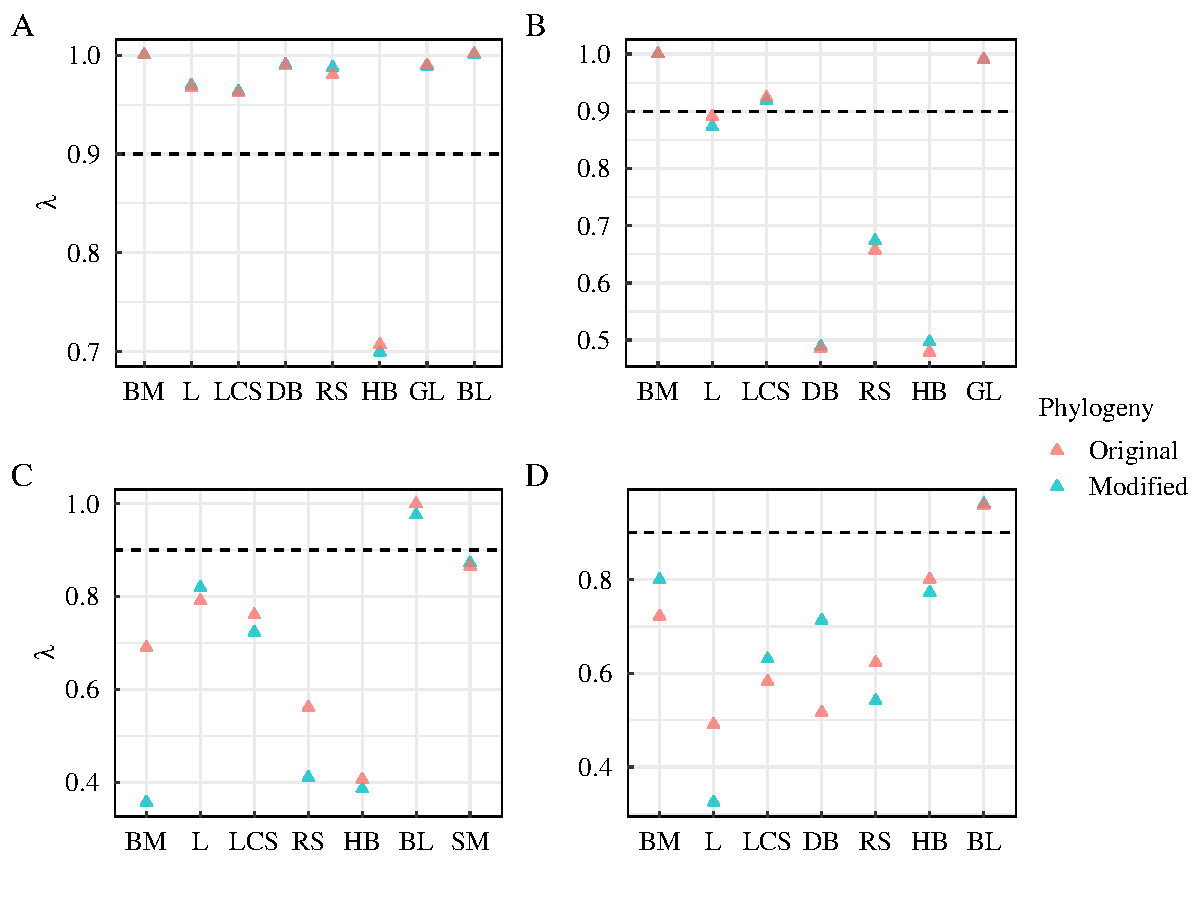
\includegraphics[scale=0.65]{figures/chapter2/Phylosignal/Continuous}
\caption[Phylogenetic signal in continuous traits (Pagel's $\lambda$) estimated with both original phylogenies and modified phylogenies]{\textbf{Phylogenetic signal in continuous traits (Pagel's $\lambda$) estimated with both original phylogenies and modified phylogenies.} \textbf{(A)} Mammals; \textbf{(B)} birds; \textbf{(C)} reptiles and \textbf{(D)} amphibians. Overall, altering the phylogenies by correcting for taxonomy and by increasing species representation did not have an important effect on $\lambda$.}
\label{signalcontinuous}
\end{figure}

\begin{figure}[h!]
\centering
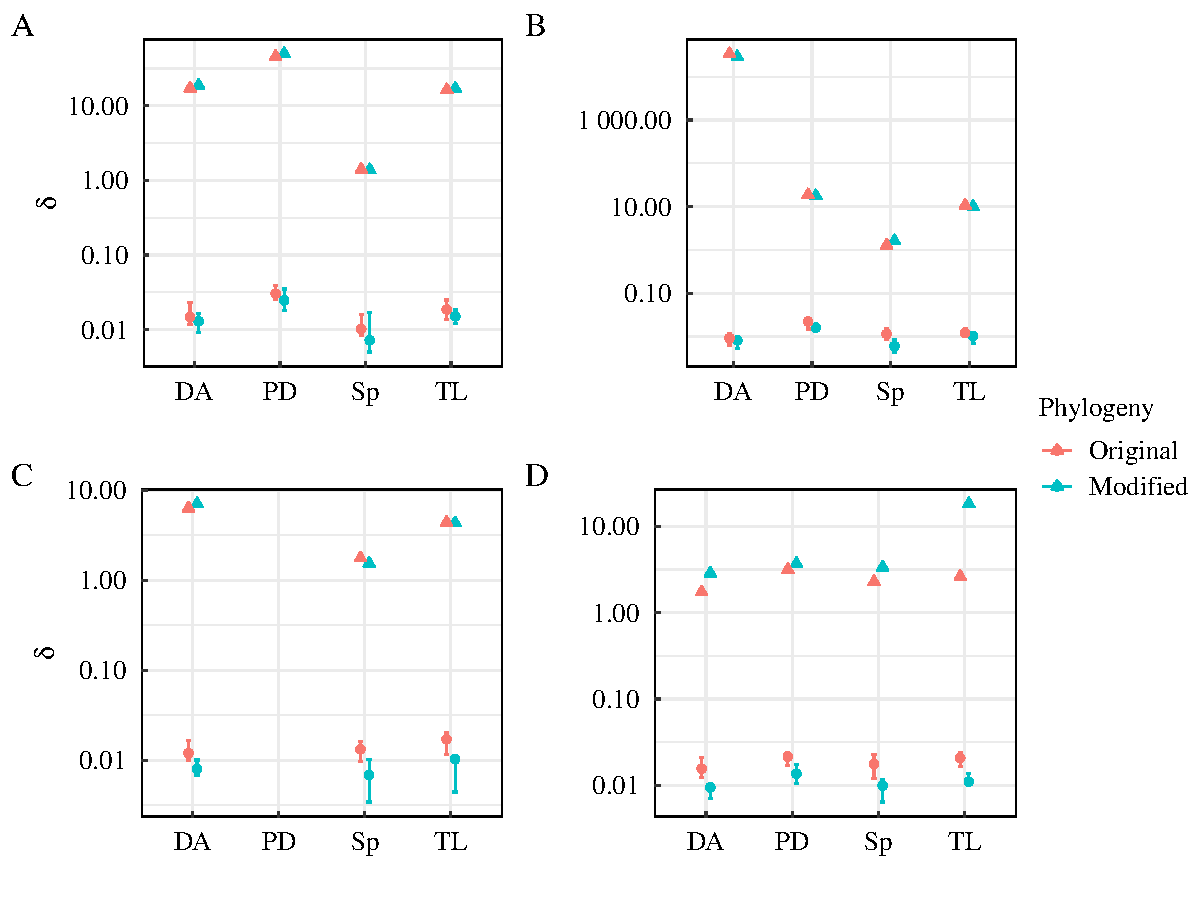
\includegraphics[scale=0.65]{figures/chapter2/Phylosignal/Categorical}
\caption[Phylogenetic signal in categorical traits ($\delta$) estimated with both original phylogenies and modified phylogenies]{\textbf{Phylogenetic signal in categorical traits ($\delta$) estimated with both original phylogenies and modified phylogenies.} \textbf{(A)} Mammals; \textbf{(B)} birds; \textbf{(C)} reptiles and \textbf{(D)} amphibians. Triangle-shaped points represent the estimated phylogenetic signal in each trait; round-shaped points represent the median null expectation of the phylogenetic signal ($\pm95\%$CI). Alterations of the phylogenies did not strongly impact $\delta$.}
\label{signalcategorical}
\end{figure}

\pagebreak


\subsubsection{Missing trait values: imputation implementation.}
Despite much variation in trait coverage across classes (see Results), the phylogenetic signal was strong in many categorical and continuous traits (Table \ref{physignal}, Figures \ref{signalcontinuous} and \ref{signalcategorical}). 
I hence imputed missing trait values using random forest algorithms, implemented by missForest. As stated above, missForest was shown by \citet{Penone2014} to be the best method when including phylogenetic information for mixed-type variable imputations. Moreover, \citet{Penone2014} also showed that adding phylogenetic information did not decrease the accuracy of imputations. 

Phylogenetic relationships were included as additional predictors in the form of phylogenetic eigenvectors \citep{Diniz-Filho2012}, extracted from the phylogenies using the PVR package \citep{Santos2018}. In this package, phylogenetic eigenvectors were computed from a phylogenetic distance matrix, and calculated using principal coordinate analysis methods. Phylogenetic eigenvectors summarised the relationships among species. \citet{Penone2014} showed that including the first 10 eigenvectors minimised the imputation error when imputing missing trait values with missForest. As such, I included the first 10 eigenvectors as additional predictors of missing trait values.

As not all species were represented in the phylogenies (Figure \ref{species_rep_phylo}), I also added taxonomic orders as an extra predictor variable in the random forest algorithm. All traits in Table \ref{datasources} were included in the imputations (except for primary diet and diet breadth in reptiles). Tuning parameters of missForest were set to 10 maximum iterations (if the stopping criterion was not met beforehand, see below) and to 100 trees grown in each forest. To further examine imputation robustness and consistency, I imputed eight datasets in parallel (eight imputed trait datasets for each class: total of 32 imputed datasets).

\subsubsection{Imputation error and robustness.}

\paragraph{Stopping criterion in missForest.}
The missForest algorithm proceeds iteratively, training random forests on sub-samples of the observed values first, then predicting missing values over several iterations. The stopping criterion is met when the difference in imputed values ($\Delta_{cont}$ and $\Delta_{cat}$, see below) between the last imputed dataset and the previously imputed dataset increases for the first time. The penultimate imputed dataset is then returned. For continuous variables, the difference $\Delta_{cont}$  is defined as:
\begin{align}
\Delta_{cont}=\frac{\sum_{j \in N}\left(X^{i,l}-X^{i,p}\right)^2}{\sum_{j \in N}\left(X^{i,l}\right)^2}, 
\end{align}
where $j$ is a continuous trait among $N$ traits, $X^{i,l}$ is the last imputed dataset and $X^{i,p}$ is the penultimate imputed dataset.  $\Delta_{cont}$ is a measure of the aggregated distance between two successive imputations across all continuous traits. For categorical variables, the difference $\Delta_{cat}$ is:
\begin{align}
\Delta_{cat}=\frac{\sum_{k \in F}\sum_{j} J_{X^{i,l}\neq X^{i,p}}}{n(NA)}, 
\label{eqPFC}
\end{align}
where $k$ is a categorical trait among $F$ categorical traits, $n(NA)$ is a the number of missing values for $k$ and $J$ is the $j^{th}$ imputed values for which the consecutive imputations predicted contradicting results. In other words, $\Delta_{cat}$ measures the proportion of values that were found to be different between two successive imputations (see \cite{Stekhoven2012} for more details). When the stopping criterion has been met,`out-of-bag' errors (OOB errors) are estimated.

\paragraph{Out-of-bag imputation error.}
OOB errors refer to errors estimated from sub-samples of the data that were not used for training the random forests (Figure \ref{OOBerrors_chart}). OOB errors are estimated from these bootstrap datasets and as such differ from `true' imputation errors, which require previous knowledge of the full dataset. The true root-mean square error (root-MSE) for continuous traits is defined as: 
\begin{align}
\sqrt{\frac{mean\left(\left(X_t-X_i\right)^2\right)}{var\left(X_t\right)}}, 
\label{true_MSE}
\end{align}
where $X_t$ is a vector of the complete trait values and $X_i$ a vector of the imputed trait values (Stekhoven 2011).

For continuous traits, the OOB error is also calculated as a mean square error (Equation \ref{true_MSE}), but using sub-samples of the data instead of the full dataset (Figure \ref{OOBerrors_chart}). For categorical traits, the OOB error is calculated as a proportion of falsely classifed values (PFC, calculated as in Equation \ref{eqPFC}), using the bootstrap sub-samples. 

\citet{Breiman2001} showed that OOB errors provide accurate proxies of the true imputation error. As such, to assess imputation accuracy, I retrieved OOB errors (OOB root-MSE and OOB PFC) across the eight imputed trait datasets in each class. I plotted the mean root-MSE and the mean PFC across the imputed datasets, as well as the range in errors across all imputed datasets.

\begin{figure}[h!]
\centering
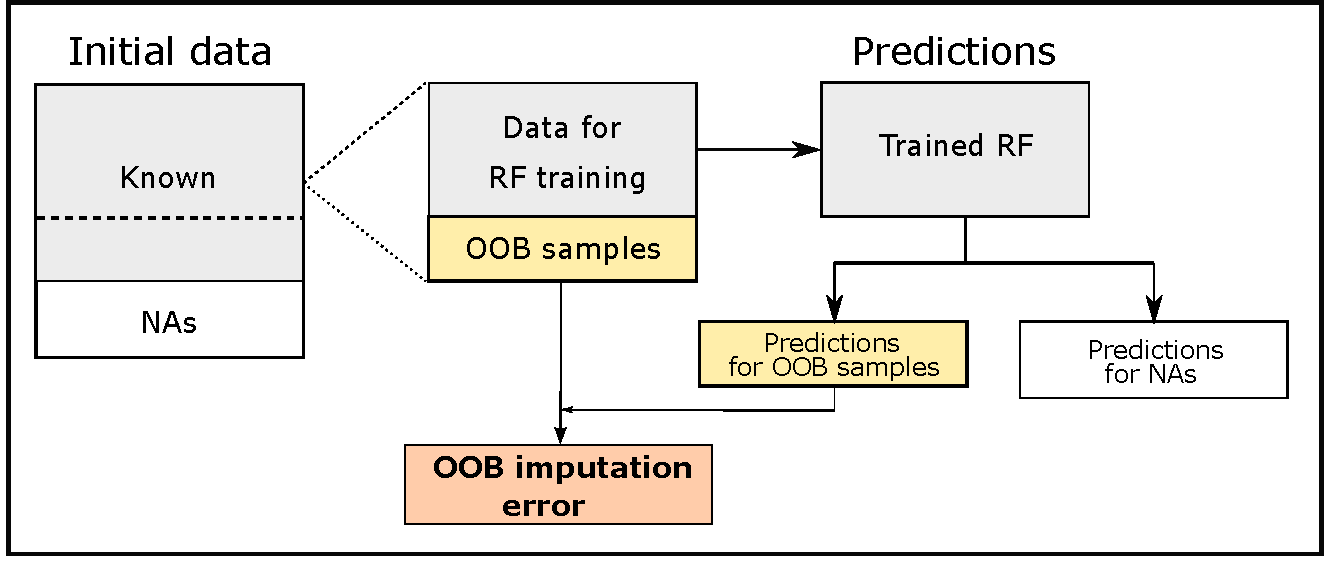
\includegraphics[scale=0.6]{figures/chapter2/OOBerror/OOB_error_chart}
\caption[Calculation of OOB errors: simplified representation of the framework]{\textbf{Calculation of OOB errors: simplified representation of the  framework.} This chart explains how OOB errors are calculated from sub-samples of the data that are not used for training the random forests. Because of the presence of missing data in the initial dataset, the true imputation error cannot be estimated. A part of the initial non-missing values are used to train the random forests. Another part (OOB samples) are reserved for estimation of OOB errors. After the random forests have been trained, values are predicted for the OOB samples and compared to the real values for these OOB samples: mean square errors and proportion of falsely classified values are calculated. OOB errors are thus estimated using sub-samples of the data. Nevertheless, OOB errors have been shown to be good proxies for true imputation errors \citep{Breiman2001}.}
\label{OOBerrors_chart}
\end{figure}

\paragraph{Imputation congruence.} To further assess whether imputations were robust, I investigated whether similar values were imputed across the eight datasets in each class, or in other words, whether results were congruent across the imputed datasets.  My expectation was that, for a trait, values imputed independently in different rounds should be nearly identical if imputations were robust. As such, for a continuous trait, pairwise correlations coefficients should be high across the eight datasets (Pearson correlation coefficients for the same trait imputed in pairwise independent rounds, see Table \ref{pairwisecorr}). For categorical traits, the random forest should predict the same values across the eight datasets. 

\begin{table}[h!]
\renewcommand{\baselinestretch}{1}
\renewcommand{\arraystretch}{1.5}
\begin{center}\fontsize{9}{11}\selectfont
\caption[Conceptual design for examining imputation congruence for continuous traits]{\textbf{Conceptual design for examining imputation congruence for continuous traits.} For one trait, pairwise correlation coefficients across eight independent imputation rounds are expected to be high if imputations are robust. To assess imputation congruence across eight imputed datasets, pairwise correlation coefficients were averaged (and the spread of the correlation coefficients assessed using the range).} 
\label{pairwisecorr}
 \begin{tabular}{c|c|c|c|}
\cline{2-4}
\multicolumn{1}{l|}{}                    & \textbf{Imputed 1} & \textbf{Imputed 2} & \textbf{Imputed n} \\ \hline
\multicolumn{1}{|c|}{\textbf{Imputed 1}} & 1                  & -                  & -                  \\ \hline
\multicolumn{1}{|c|}{\textbf{Imputed 2}} & corr(1,2)          & 1                  & -                  \\ \hline
\multicolumn{1}{|c|}{\textbf{Imputed n}} & corr(n,1)          & corr(n,2)          & 1                  \\ \hline
\end{tabular}
\end{center}
\end{table}


For continuous traits, I assessed imputation congruence across the eight imputed datasets by averaging pairwise Pearson correlation coefficients and plotting the mean (and range) for each trait. For categorical traits, I assessed congruence by assessing the percentage of species for which all eight imputed values were identical.

\section{Results}

\subsection{Outputs}
I collected and imputed data for nine traits, plus range size, across 11637 avian species, 5502 mammalian species, 10334 reptilian species and 6904 amphibian species. Datasets recording species synonymic binomial names were also produced. 

\subsection{Biases in the availability of trait information: patterns in missing trait values}

\subsubsection{Increases in coverage and completeness due to taxonomic corrections.} 
%Figure \ref{traitcov} shows the trait coverage within each class and for each trait, before and after correcting for taxonomy. Figure \ref{traitcomp} shows the distribution of trait completeness before and after taxonomic corrections, as well as the median trait completeness for each class.
Across all classes, correcting for taxonomy increased trait coverage (Figure \ref{traitcov}). Nevertheless, the increase in coverage for reptiles was marginal, which may indicate that the procedure developed to extract and identify accepted names overall performed less well for reptilian species than for mammals, birds and amphibians. Similarly, correcting for taxonomy improved trait completeness in all classes, although less so for reptiles (Figure \ref{traitcomp}). Wilcoxon rank sum tests, testing the null hypothesis that uncorrected and corrected completeness distributions came from the same population, rejected this hypothesis across all classes (alternative hypothesis: uncorrected medians were lower than corrected medians; mammals: p-value=1.2$\cdot10^{-9}$; birds: p-value<2.2$\cdot10^{-16}$; reptiles: p-value=0.025; amphibians: p-value<2.2$\cdot10^{-16}$). To conclude, correcting for taxonomy had a significant impact on trait completeness, and increased coverage in most cases. 


\begin{figure}[h!]
\centering
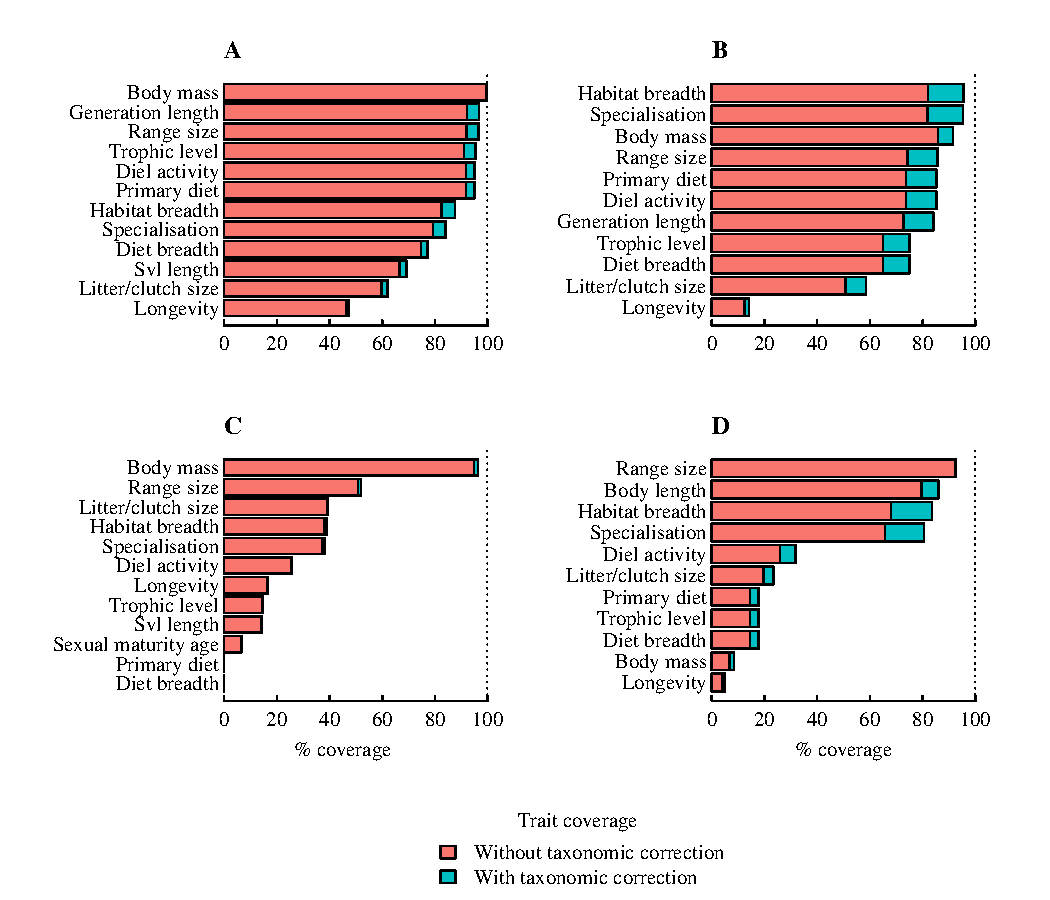
\includegraphics[scale=0.85]{figures/chapter2/Trait_coverage/Predictor_traits/All_species}
\caption[Trait coverage across all species before and after taxonomic correction]{\textbf{Trait coverage across all species before and after taxonomic correction.} Here are shown target traits as well as a few other traits used in imputations as additional predictors (such as generation length for mammals and birds or body length for amphibians). \textbf{(A)} Mammals (5885 species before correction, 5502 after correction); \textbf{(B)} birds (13554 species before correction, 11637 after correction); \textbf{(C)} reptiles (10722 species before correction, 10334 after correction) and \textbf{(D)}  amphibians (8643 species before correction, 6904 after correction). Trait coverage was calculated as the percentage of species for which trait information was available. Correcting for taxonomic synonymy improved coverage in most cases. For mammals and birds, all traits had an initial coverage of more than 50\%, except longevity (but generation lengths were estimated for most species). On the other hand, trait coverage was poor (below 50\%) for 80\% of all reptilian traits, and for 64\% of all amphibian traits.}
\label{traitcov}
\end{figure}

\subsubsection{Taxonomic biases in the availability of trait information: exacerbated Raunki{\ae}r shortfall in reptiles and amphibians.}

\paragraph{Trait coverage.}
Trait coverage was highly variable across classes and traits. Trait coverage was initially good for most mammalian and avian traits, which had more than 50\% coverage (Figure \ref{traitcov} A and B). Only longevity had a coverage lower than 50\% for these classes, although generation length was above 80\% in both cases (longevity and generation length being closely related). Conversely, trait coverage was overall much poorer for reptiles and amphibians (Figure \ref{traitcov} C and D): 64\% of amphibian traits and 80\% of reptilian traits presented a coverage below 50\%.  
Although amphibians and reptiles appeared to be less sampled in many traits, body mass/body length information, range size and habitat variables (in amphibians only) presented coverages above 80\%.

As such, contrasting patterns of trait coverage appeared between, on the one hand, mammals and birds, and on the other hand, amphibians and reptiles, highlighting the existence of taxonomic biases in data collection. For species found in PREDICTS only, coverage increased disproportionally in reptiles and amphibians compared to the coverage for the full set of species (the figure for PREDICTS species only is available in the SI).

\paragraph{Trait completeness.}
Trait completeness (the proportion of traits sampled for a given species) reflected similar biases as trait coverage (Figure \ref{traitcomp}). The median completeness with taxonomic correction was high for mammals and birds (92\% and 82\% respectively) but much lower for reptiles and amphibians (30\% and 36\% respectively). A pairwise Kruskall-Wallis rank sum test rejected the hypothesis that completeness distributions across classes originated from the same distribution (p-values<2$\cdot10^{-16}$ in all cases), showing that the availability of trait information varied significantly among classes. 

\begin{figure}[h]
\centering
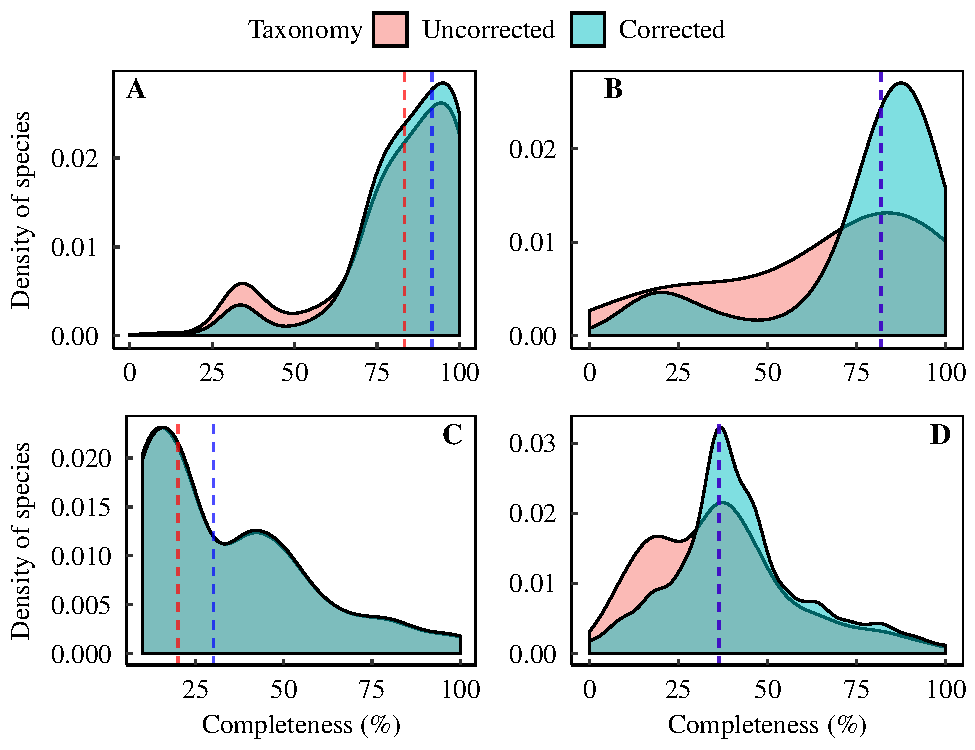
\includegraphics[scale=0.70]{figures/chapter2/Trait_coverage/Missing_values/Traitcompleteness}
\caption[Distribution of completeness of trait information across species]{\textbf{Distribution of completeness of trait information across species.} For a given species, completeness was calculated as the proportion of traits that were estimated (non-missing value). Completeness was calculated here over the same set of traits shown in Figure \ref{traitcov} (all predictor traits). \textbf{(A)} Mammals; \textbf{(B)} birds; \textbf{(C)} reptiles and \textbf{(D)} amphibians. Correcting for taxonomy affected completeness, significantly shifting the distributions to the right (alternative hypothesis, Wilcoxon rank sum tests: uncorrected medians were lower than corrected medians; mammals: p-value=1.2$\cdot10^{-9}$; birds: p-value<2.2$\cdot10^{-16}$; reptiles: p-value=0.025; amphibians: p-value<2.2$\cdot10^{-16}$). The availability of trait information varied significantly among classes (a pairwise Kruskall-Wallis rank sum test rejected the null hypothesis that completeness distributions across classes originated from the same distribution (p-values<$2\cdot10^{-16}$ in all cases)).}
\label{traitcomp}
\end{figure}


\newpage
\subsubsection{Non-randomness in trait information: phylogenetic biases.}

\paragraph{Phylogenetic patterns of trait completeness.}
As expected from the distributions of completeness values for mammals and birds, within-family completeness was high across most branches of the phylogenetic trees (Figure \ref{classcomp} A and B). In herptiles, nevertheless, clusters of similar completeness appeared at family levels (Figure \ref{classcomp} C and D).
For better visualisation, the trees were represented without tip labels. Figures providing tip labels are available in the SI (for each class, tip label information includes taxonomic order and family; zooming in the figures may be required). 

In mammals, chiropterans appeared to have lower median trait completeness than other orders (light blue cluster appearing in the middle of the tree, located with $*$ on the plot, Figure \ref{classcomp} A). Species in the Diprotodontia order (marsupials: kangaroos, wallabies, koalas and their relatives) were particularly well sampled, as well as carnivorans, and some families in the Cetartiodactyla order (ungulates such as bovids, giraffes or deer).

In birds, Procellariiformes (albatrosses, petrels, shearwaters and their relatives), Charadriiformes (sandpipers, plovers, gulls, auks, and their relatives), and Anseriformes (screamers, ducks, geese and their relatives) appeared to be particularly well sampled (Figure \ref{classcomp} B). 

In reptiles (Figure \ref{classcomp} C), most lizards and amphisbaenians  
showed moderate completeness ($\sim$50\%). Some families of lizards were well sampled (such as the beaded lizards of the Helodermatidae family, or the casquehead lizards of the Corytophanidae family). Most snakes were poorly sampled: two clusters of families appeared to have low completeness. These clusters comprised species such as blind snakes of the Typhlopidae family or colubrids. A cluster of snakes comprising pythons and boas showed moderate completeness. \textbf{NB:} The phylogeny only included squamates.

In amphibians, groups of families in the Anura order (frogs) showed both the best and worst median completeness (Figure \ref{classcomp} D). For instance, the best sampled families included Leiopelmatidae (four species endemic to New Zealand), or the tailed frogs (Ascaphidae family, occurring in North America). The best sampled families also included species in the Caudata order, such as giant salamanders (Cryptobranchidae family). On the other hand, species in the Ranidae family (true frogs) figured among the worse sampled families, as well as, for example, the shrub frogs (Rhacophoridae). 

\begin{figure}[h!]
\centering
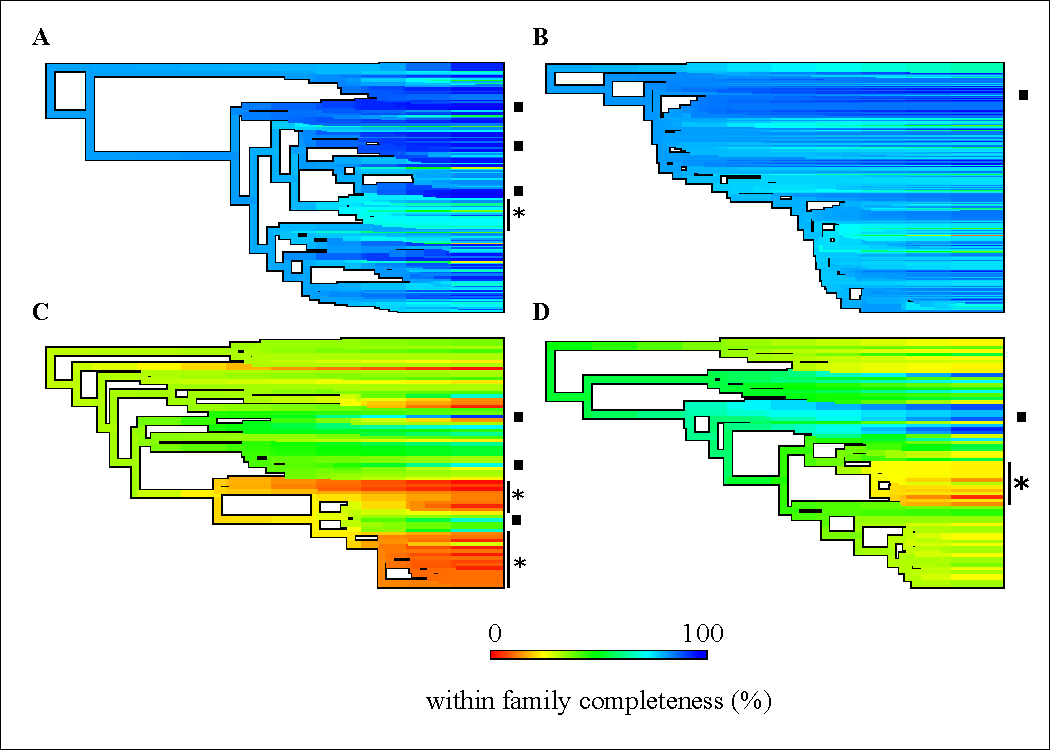
\includegraphics[scale=0.9]{figures/chapter2/NA_phylo_patterns/Completeness_all_2}
\caption[Median completeness across families]{\textbf{Median completeness across families.} Tips labels are not shown here for better visualisation of the results; the same figures with tip labels are provided in the SI (zooming into the figure is necessary for mammals and birds); tip label information includes order and family.
Stars indicated clusters of families identified to be less well sampled. Squares represent the approximate location of some families, or some groups of families, that show high trait completeness. \textbf{(A)} Mammals. From top to bottom, the highlighted groups are: marsupials; carnivorans; ungulates; chiropterans.  \textbf{(B)} Birds. The highlighted group includes petrels, albatrosses, gulls, ducks,  and plovers. \textbf{(C)} Squamates. From top to bottom, the highlighted groups are: beaded lizards; casquehead lizards; cluster of snakes (comprising some blind snakes of the Typhlopidae family); cluster of snakes comprising boas and pythons; cluster of snakes (comprising colubrids). \textbf{(D)} Amphibians. The first highlighted group comprises well sampled families of frogs such as Leiopelmatidae (four species endemic to New Zealand) and the tailed frogs. The second group is a cluster of poorly sampled frogs including true frogs and shrub frogs.}
\label{classcomp}
\end{figure}

Overall, these results showed that median trait completeness was not distributed randomly across the tree branches. Closely related families seemed to share more similar median trait completeness than less closely related families. This was particularly emphasized in reptiles and amphibians.

\newpage

\paragraph{Phylogenetic patterns of trait missingness.}
As trait missingness decreased, family clusters of similar median trait missingness became more visible (Figures \ref{familycov_mammals}, \ref{familycov_birds}, \ref{familycov_reptiles} and \ref{familycov_amphibians}). In mammals, a cluster of families showed low median missingness for trophic level; most of these families belonged to the Cetartiodactyla order, which contained aquatic mammals. Chiropterans appeared to be less well sampled for three traits compared to other orders (body length, litter size, longevity, subplots J to L, Figure \ref{familycov_mammals}). Primates also appeared to be less well sampled for certain traits (subplots E to I). Among the best sampled groups were the marsupials and the carnivorans.

For birds, the patterns were less clear (Figure \ref{familycov_birds}). For low percentages of trait missingness (subplots A to G), within-family trait missingness values seemed to be distributed randomly across branches. Diet information was less resolved for Struthioniformes (ostriches and their relatives, subplots H and L: green cluster). Overall, no systematic bias emerged.

In squamates (Figure \ref{familycov_reptiles}), snakes were systematically less well sampled for a number of traits (subplots C to J), with a few exceptions for families that included boas and pythons (subplot C to H: green-blue areas within the red cluster). Overall, trait information for most snakes was systematically less well complete than for other squamates.

In amphibians (Figure \ref{familycov_reptiles}), many frog families were systematically less well sampled for a number of traits (subplots C, D and to K). On the other hand, other frog families were the best sampled families for similar traits (blue clusters on subplots E to L). Families of the Gymnophonia order (comprising caecilians) were also systematically less well sampled for many traits (top red cluster in subplot K).

% Mammals
\begin{figure}[]
\centering
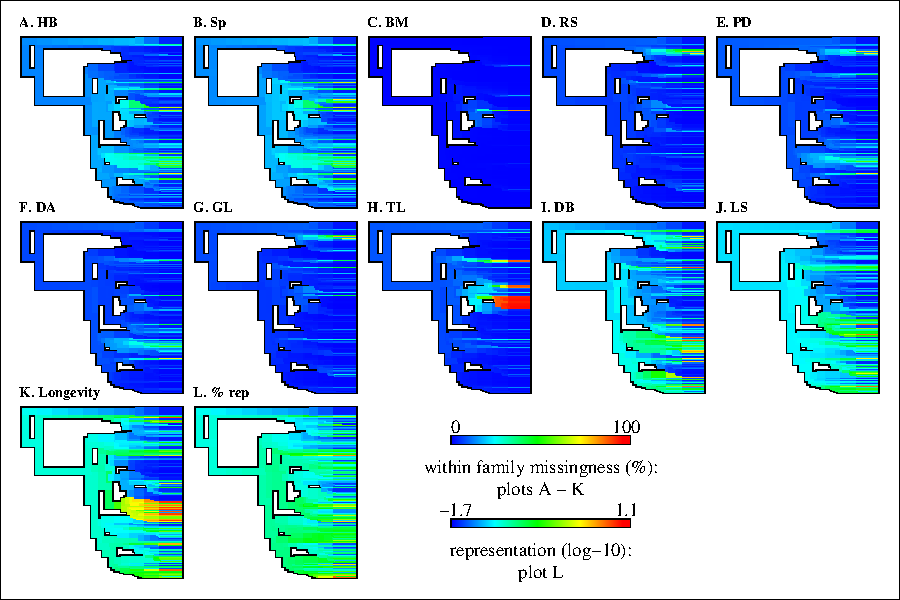
\includegraphics[scale=1.1]{figures/chapter2/NA_phylo_patterns/Mammals_coverage}
\caption[Within-family median trait missingness in mammals]{\textbf{Within-family median trait missingness in mammals.} The subplots are ordered from the trait showing highest overall coverage to the trait showing lowest overall coverage. The last subplot (`\%rep') represents the contribution of each family to the total number of species in the phylogeny. \textbf{BM:} body mass; \textbf{GL:} generation length; \textbf{RS:} range size; \textbf{TL:} trophic level; \textbf{DA:} Diel activity; \textbf{PD:} Primary diet; \textbf{HB:} Habitat breadth; \textbf{Sp:} Natural habitat specialisation; \textbf{DB:} diet breadth; \textbf{BL:} body length; \textbf{LCS:} litter/clutch size. Chiropterans appeared to be less well sampled for three traits (body length, litter/clutch size, and longevity). Primates also appeared to be less well sampled for a number of traits (light green cluster on subplots E to I). The red cluster on subplot D corresponds to the Cetartiodactyla order, which contained aquatic mammals. Carnivorans and marsupials were better sampled for most traits. }
\label{familycov_mammals}
\end{figure}

\clearpage
% Birds
\begin{figure}[]
\centering
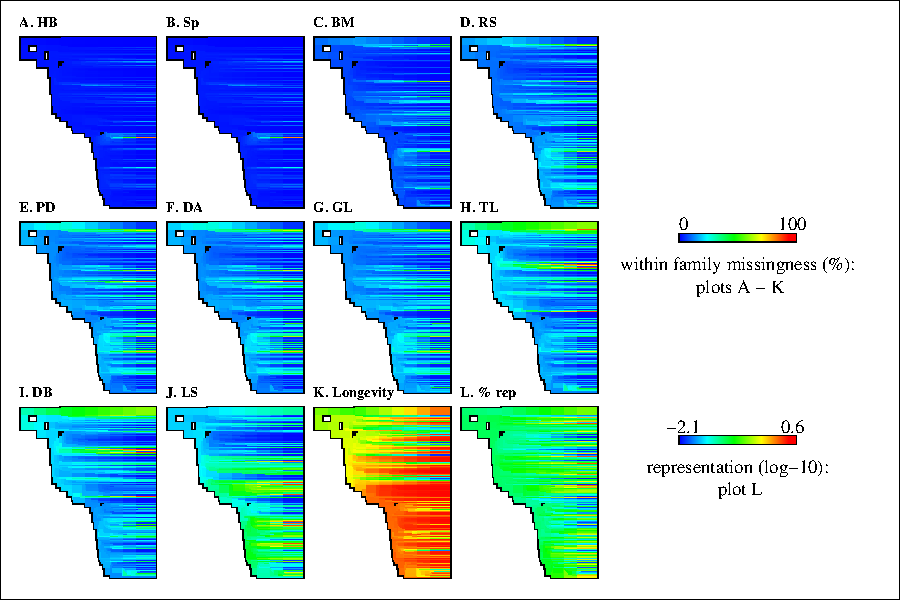
\includegraphics[scale=1.1]{figures/chapter2/NA_phylo_patterns/Birds_coverage}
\caption[Within-family median trait missingness in birds]{\textbf{Within-family median trait missingness in birds.} The subplots are ordered from the trait showing highest overall coverage to the trait showing lowest overall coverage. The last subplot (`\%rep') represents the contribution of each family to the total number of species in the phylogeny. \textbf{HB:} Habitat breadth; \textbf{Sp:} Natural habitat specialisation; \textbf{BM:} body mass; \textbf{RS:} range size; \textbf{PD:} Primary diet; \textbf{DA:} Diel activity; \textbf{GL:} generation length;  \textbf{TL:} trophic level; \textbf{DB:} diet breadth; \textbf{LS:} litter/clutch size. No systematic bias emerged in trait sampling for birds.}
\label{familycov_birds}
\end{figure}

\clearpage
% Reptiles
\begin{figure}[]
\centering
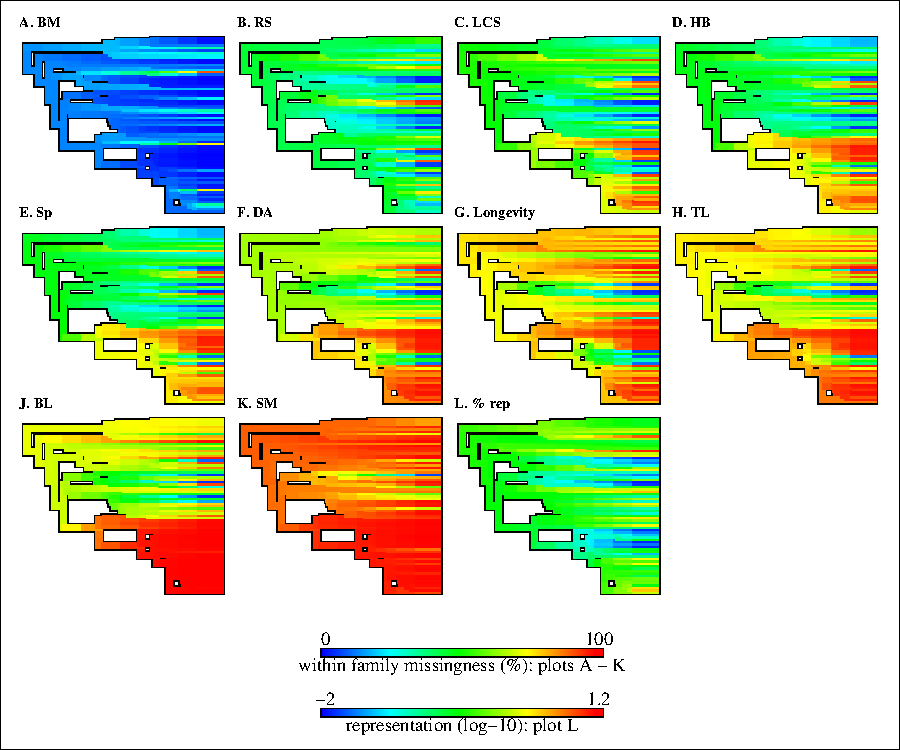
\includegraphics[scale=1.1]{figures/chapter2/NA_phylo_patterns/Reptiles_coverage}
\caption[Within-family median trait missingness in squamates]{\textbf{Within-family median trait missingness in squamates.} The subplots are ordered from the trait showing highest overall coverage to the trait showing lowest overall coverage. The last subplot (`\%rep') represents the contribution of each family to the total number of species in the phylogeny. \textbf{BM:} body mass; \textbf{RS:} range size; \textbf{LCS:} litter/clutch size; \textbf{HB:} Habitat breadth; \textbf{Sp:} Natural habitat specialisation; \textbf{DA:} Diel activity; \textbf{TL:} trophic level; \textbf{BL:} body length; \textbf{SM:} sexual maturity age. Snakes were systematically less well sampled for a number of traits (subplots C to J) -- except for families comprising boas, pythons and their relatives.}
\label{familycov_reptiles}
\end{figure}

\clearpage
% Amphibians
\begin{figure}[]
\centering
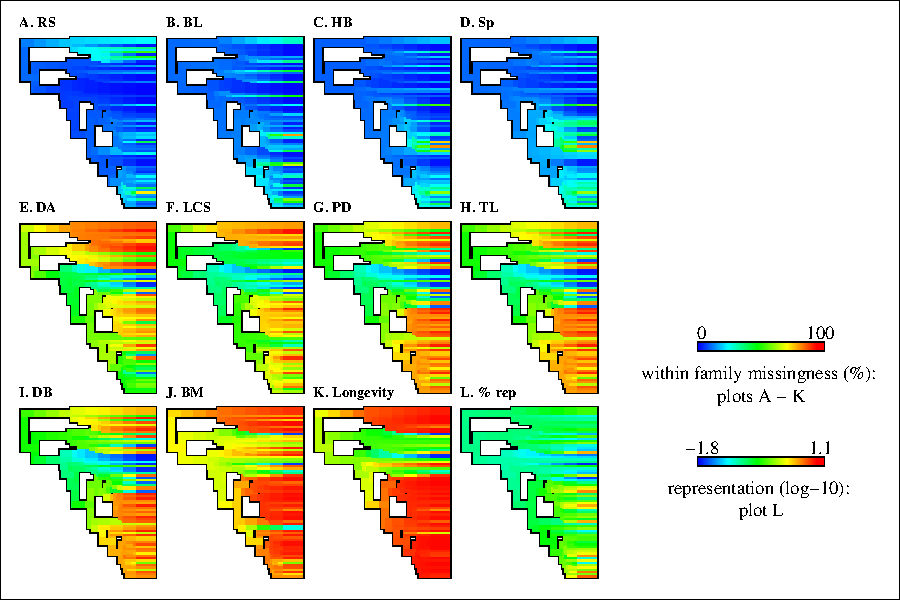
\includegraphics[scale=1.1]{figures/chapter2/NA_phylo_patterns/Amphibians_coverage}
\caption[Within-family median trait missingness in amphibians]{\textbf{Within-family median trait missingness in amphibians.} The subplots are ordered from the trait showing highest overall coverage to the trait showing lowest overall coverage. The last subplot (`\%rep') represents the contribution of each family to the total number of species in the phylogeny. \textbf{RS:} range size; \textbf{BL:} body length; \textbf{HB:} Habitat breadth; \textbf{Sp:} Natural habitat specialisation; \textbf{DA:} Diel activity; \textbf{LCS:} litter/clutch size; \textbf{PD:} Primary diet; \textbf{TL:} trophic level; \textbf{DB:} Diet breadth; \textbf{BM:} body mass. Frogs were overall systematically less well sampled (subplots C, D, K), as well as families in the Gymnophonia order (caecilians and their relatives: top red cluster in subplot K). Nevertheless, frog families also figured among the best sampled families (subplots E to L).}
\label{familycov_amphibians}
\end{figure}

\clearpage
\subsection{Spatial biases of trait completeness} 
Geographical range size had a significant effect on the number of sampled traits: species with larger geographical range sizes had higher trait completeness (Figure \ref{poisson}). Nevertheless, the rate of increase differed across classes. Class had a significant effect on the rate of increase of trait completeness except for reptiles (the rate of increase for reptiles was similar to the rate of increase for amphibians). Baseline rates were higher for mammals and birds than for herptiles, but rates of increase were higher for herptiles. The model coefficients, standard errors and p-values are provided in the SI.
%A goodness-of-fit test on the residual deviance did not gather evidence that the model fitted badly (p=1, residual deviance: 14440 on 27105 degrees of freedom).
% develop this paragraph and add results for goodness-of-fit

\begin{figure}[h!]
\centering
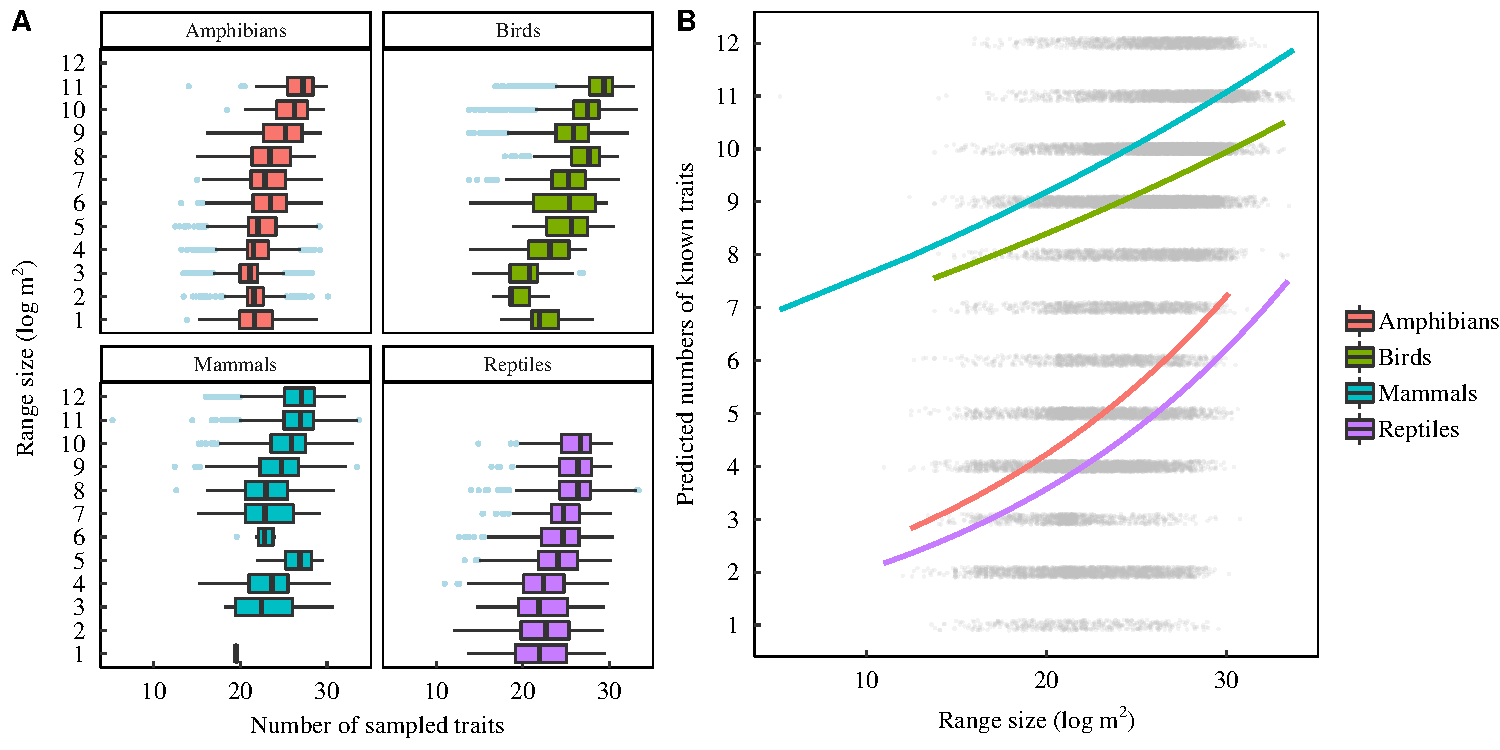
\includegraphics[scale=0.7]{figures/chapter2/NA_spatial_patterns/Poisson_model_predictions}
\caption[Relationship between trait completeness and species geographical range size]{\textbf{Relationship between trait completeness and species geographical range size.} \textbf{(A)} Boxplots showing the number of traits sampled in each class against species geographical range sizes (log$_{10}$). \textbf{(B)} Regression lines for the fitted generalised linear model. Grey points represent empirical values (not colour coded for better visual clarity). The model was fitted using a Poisson error distribution. Class was added as an explanatory variable interacting with range size.}
\label{poisson}
\end{figure}


\subsection{Imputation performance and robustness}

\subsubsection{Out-of-bag imputation errors.}
Figure \ref{OOBerrors} A shows OOB root-mean-square errors for each continuous traits (shown here for one randomly selected imputed dataset). Figure \ref{OOBerrors} B is the OOB proportion of falsely classified values for categorical traits (for the same imputed dataset).
Estimated prediction errors for categorical traits were low to moderate (all below 20\%). For continuous traits, estimated errors could be large (e.g., mammalian body mass, amphibian clutch size  or range sizes). Nevertheless, such large errors were driven by high trait values in the dataset (see Figure \ref{traitdist}, which shows the distribution of trait values after imputations; large prediction errors are estimated where traits can attain high values). 
 
\begin{figure}[h!]
\centering
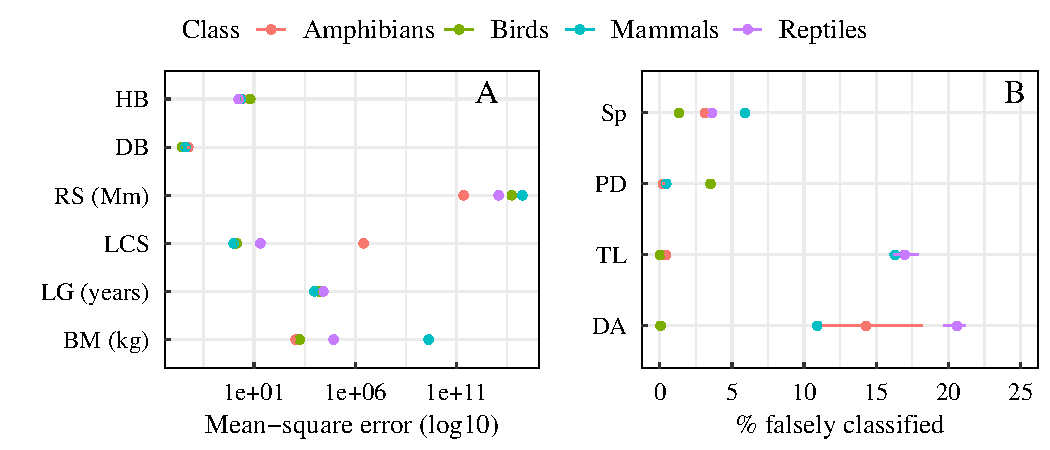
\includegraphics[scale=0.75]{figures/chapter2/Imputation_errors/MSE_PFC}
\caption[missForest out-of-bag root-mean-square errors and proportion of falsely classified values]{\textbf{missForest out-of-bag root-mean-squared errors and proportion of falsely classified values.} \textbf{(A)} Out-of-bag root-mean-square errors for continuous traits. \textbf{(B)} Out-of-bag proportion of falsely classified values.}
\label{OOBerrors}
\end{figure}

\begin{figure}[h!]
\centering
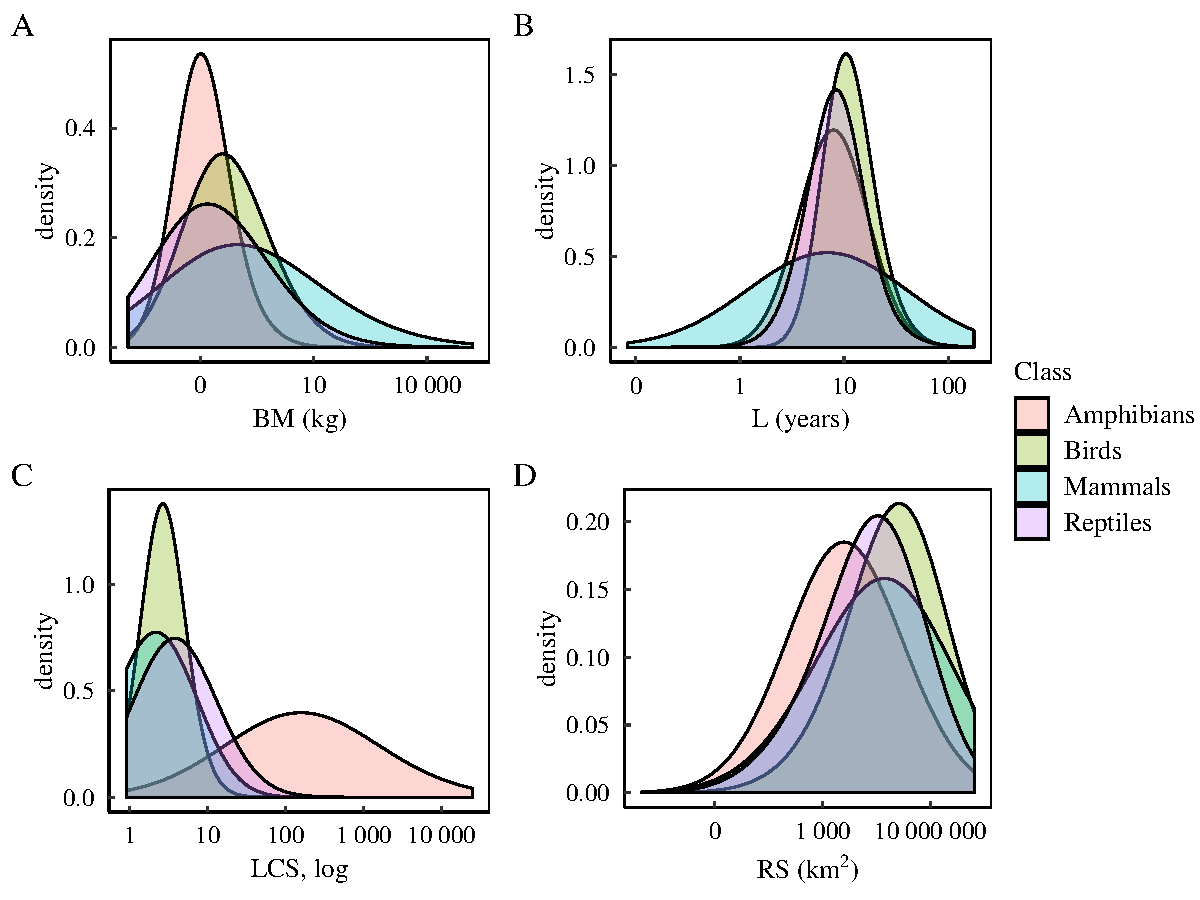
\includegraphics[scale=0.7]{figures/chapter2/Imputation_errors/Distributions}
\caption[Distribution of trait values after imputation for body mass, longevity, litter/clutch size and distribution of range sizes]{\textbf{Distribution of trait values after imputation for body mass, longevity, litter/clutch size and distribution of range sizes.}}
\label{traitdist}
\end{figure}


\pagebreak
\subsubsection{Congruence of imputed values among eight imputed datasets.}

Figure \ref{congruence} A shows the range and mean of pairwise correlation coefficients obtained for each continuous trait, across eight imputed datasets. Pairwise correlation coefficients were calculated for each trait, predicted in eight independent imputation rounds, so that high correlation  values indicated more similar predictions for one trait across the eight datasets. Overall, imputation congruence was high for all continuous traits except habitat breadth. Imputation congruence was high across all classes for longevity (minimum mean correlation coefficient of 0.87 for reptiles), but more variable in other traits depending on the class.

Figure \ref{congruence} B shows the proportion of species for which imputed values were identical across the eight imputed datasets (for categorical traits). At least 50\% of all species had identical predicted values across all imputed traits. Imputation congruence was high for trophic level (above 86\% in all classes), and more variable in other traits depending on the class. 

Mammals had the best imputation congruence scores in both continuous and categorical traits (minimum mean correlation coefficient of 0.85 for continuous traits and minimum percentage of agreement of 85\% for categorical traits). Imputation congruence for birds was also very good, though scores were slightly lower for diet related variables (diet breadth and primary diet). For amphibians and reptiles, mean correlation coefficients were all above 0.60, except for habitat breadth. For amphibians in particular, imputation congruence on habitat breadth was poor. Overall, imputed results for amphibians were less congruent than for reptiles, birds and mammals.

\begin{figure}[h!]
\centering
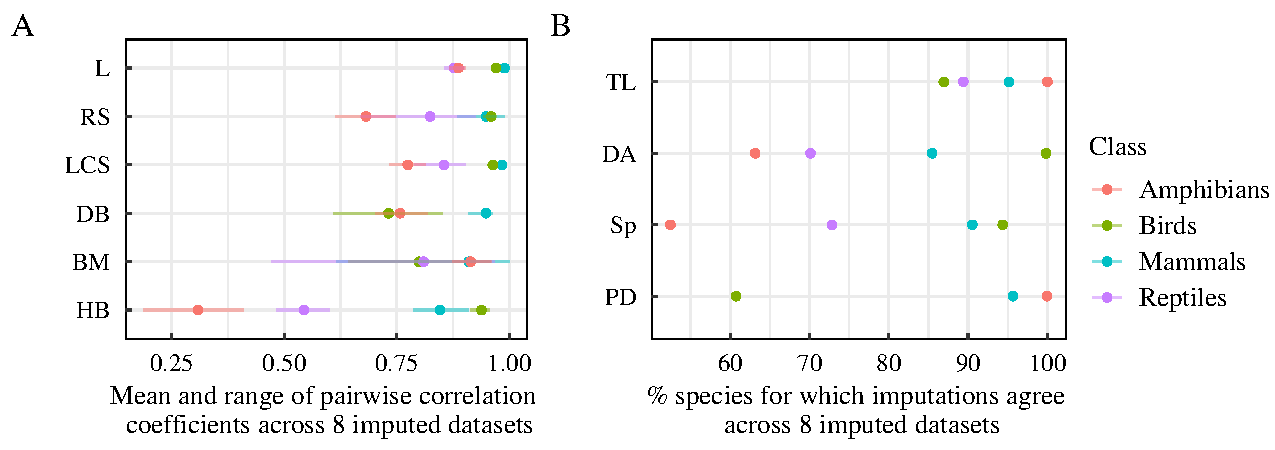
\includegraphics[scale=0.75]{figures/chapter2/Congruence_imputations/Summary}
\caption[Imputation congruence across eight imputed datasets]{\textbf{Imputation congruence across eight imputed datasets.} \textbf{(A)} Mean of pairwise correlation coefficients for continuous traits; \textbf{(B)} proportion of species for which all imputed values were congruent. Imputation congruence was overall good for categorical traits (all above 50\%). The lowest scores were obtained for primary diet in birds, as well as for diel activity and specialisation in both reptiles and amphibians (the four points below 85\% in \textbf{(B)}). For continuous traits, the means of all pairwise correlation coefficients were above 50\%, except for amphibian habitat breadth. The SI provide more detailed congruence results (plots for each class and each trait).}
\label{congruence}
\end{figure}

OOB imputation errors and imputation congruence showed that predictions were overall robust. Habitat breadth was the only variable for which imputation congruence was highly variable across classes, and below 50\% for amphibians. Imputation accuracy may be impacted by the phylogenetic biases in trait completeness. Further work could investigate the impact of phylogenetic non-randomness in the sampling of trait values on imputation accuracy. 

\section{Discussion}
% explain what trait baises could mean for the real world.

In this work, I compiled and imputed data on 10 traits across 5502 mammalian, 10334 reptilian, 11637 avian and 6904 amphibian species. Traits related to species morphological characteristics (body mass), to their life-history (litter/clutch size, longevity, diel activity), to their habitat preferences (habitat breadth, specialisation), and to their diet (trophic level; for mammals, birds and amphibians only, primary diet and diet breadth were also collated). To my knowledge, there is yet no published or freely available trait database encompassing all terrestrial vertebrates. As such, this work could constitute one of the first attempts to collate extensive trait information across all terrestrial vertebrates, which was enabled by all past and recent efforts to release trait information in the public domain (e.g. PanTHERIA: \citet{Jones2009}; Amniote database: \citet{Myhrvold2015}; AmphiBIO: \citet{Oliveira2017}, EltonTraits: \citet{Wilman2014}; MammalDIET: \citet{Kissling2014}; and many other datasets, Table \ref{datasources}). Note that the current imputed dataset contains fossil species, as some of the primary sources provided estimates for these. Some marine and aquatic mammals are also represented. Both fossil and non-terrestrial species could be filtered out if necessary in the course of my PhD.

Further developments could include enhancing the existing data to improve initial trait coverage. If novel primary sources were released, new variables could be added to the dataset. Even though the traits included in this work already encompass most of the ecological traits available in the literature across vertebrate classes, one notable omission was species mobility. Species abilities to both move within their habitats (home range) and to disperse and colonise new areas has a major impact on their aptitudes to cope with anthropogenic changes and on ecosystem functions \citep{Tucker2018, Schloss2012}. Nevertheless, traits relating to mobility in amphibians or reptiles were unavailable. The only readily available variable that could have been added was volancy. Another important information that could further enhance the dataset is reptilian diet, which would require important data collection efforts. For all classes, the dataset could be extended with thermal regulation aptitudes (endothermy VS ectothermy), as well as foraging strata and terrestriality (species habitat preferences along a vertical gradient: e.g. above versus below ground preferences).

% biases in trait information
The data collection revealed important biases in the availability of trait information across terrestrial vertebrates. The data was taxonomically biased, with better completeness of trait information in mammals and birds, even when species had similar range sizes. Species with bigger geographical range sizes were more likely to have more complete trait information. The effect of geographical range size was more pronounced for herptiles than for mammals and birds, with steeper decreases in completeness with decreasing range sizes. In herptiles, trait information was strongly phylogenetically biased;  entire clades appeared to be systematically less well sampled. These results illustrate the biases in global biodiversity knowledge identified by \citet{Hortal2014}. Identified gaps are consistent with biases found in \citet{Gonzalez-Suarez2012} (study conducted on mammals only). 

Such biases in trait information have important consequences for conservation.  Narrow-ranged species are less well sampled than widespread species, which could be make conservation planning more difficult for narrow-ranged species.
Nevertheless, narrow-ranged species have higher extinction risks than widespread species \citep{Collen2016, Purvis2000, Ripple2017}, are more negatively impacted by anthropogenic disturbances \citep{Newbold2018a}, and can support unique ecosystem functions \citep{Mouillot2013}. The biases in trait data hence show that information is less available when potentially more critical to conservation planning. Further work could investigate in more details the spatial biases in trait information, for instance by comparing trait data available for temperate species and for tropical species. Indeed, tropical areas are hyperdiverse areas of critical importance for worldwide conservation \citep{Barlow2018}. 

Biases in trait information also have consequences for macro-ecological studies. For instance, some analyses make inferences from taxa for which data is available, to other missing-value taxa. Nevertheless, if the sample of non-missing data species is not representative, due to biases in sampling, extrapolations may not be valid, as estimates may be biased. As such, there is a risk of biasing datasets when dropping missing data \citep{Nakagawa2008}. Imputing missing values therefore appeared to be an interesting option; nevertheless, phylogenetic non-randomness in missing values could have affected imputation accuracy.

\citet{Penone2014} conducted a simulation study where missing values were introduced in a trait dataset (10 to 80\% missing values). Values were removed in three different ways: completely at random; at random with respect to only one trait; and finally, at random with respect to phylogenies. Their results showed that differences in imputation error in these three cases were marginal and not significant. For some traits, there was a trend for bigger imputation error where missing data were clustered in closely related species.  Nevertheless, \citet{Penone2014} showed that missForest imputations were robust even when trait data was phylogenetically biased.  

% using random forests and need to assess imputation acurracy
Using non parametric random forest algorithms to impute missing trait values, as implemented in R by the missForest function, presented several advantages over other imputation methods. First, random forests could deal with mixed type variables, and estimate OOB errors for each variable. Second, no underlying data distribution was assumed in the process. Third, missForest was computationally faster than other methods, which was an important criterion. Finally, missForest has been shown to outperform or perform as well as other approaches \citep{Stekhoven2012, Penone2014}. Moreover, as stated above, \citet{Penone2014} showed that missForest imputations were robust even when  missing values were not missing at random. Congruence results and imputation errors obtained here showed that missForest performed overall rather well. Habitat related variables showed less congruence and may as such be more difficult to impute. Notably, the lowest congruence was observed for habitat breadth. This may be due to the fact that the phylogenetic signal for habitat related variables was less strong (Table \ref{physignal}). Habitat related variables could be as such more difficult to explain and predict on the basis of the phylogenetic relatedness of species. Moreover, habitat related variables are not expected to correlate strongly with many other traits, so that less pertinent predictors may be available for these variables than for other traits.

This work highlighted several frequent issues met when working with a large number of species or when working with datasets from different origins. For categorical variables, the levels of the least resolved dataset had to be adopted across all classes, even though more detailed information was available in another class. Indeed, common denominators had to be found, at the expanse of highly resolved data. One example was diel activity time, that I had to constrain to two categories (nocturnal or non-nocturnal).

I also did not compile any metric reflecting intra-specific variability in continuous traits. Intra-specific variability has been shown to have important effects on ecological systems \citep{DesRoches2018, Bolnick2011, Gonzalez-Suarez2013a}. A growing body of literature encourages trait-based research to include intraspecific variability \citep{Carmona2016, Violle2012}. Here, metrics reflecting intraspecific variability were excluded due to both the scale of the data compilation and the lack of estimates across classes.

% taxonomic replication
One major issue in this work was the taxonomic redundancy of species due to the presence of similar species under diverse names, and other taxonomic errors. Here, taxonomic synonymy artificially increased the amount of missing trait values by creating `replicates' of the same species, inflated the overall number of species and significantly lowered median trait completeness. Taxonomic uncertainty is a recurring problem in ecology and conservation \citep{Isaac2004}. For instance, \citet{Cardoso2017} showed than taxonomic inaccuracies and errors in species checklists lead to the overestimation of plant diversity in the Amazon. The lack of a universal, standardised database for species names complicates species identification. Nevertheless, the production of such a database is difficult to achieve, partly because different conceptual definitions of what a species is can lead to different taxonomic systems \citep{Isaac2004}. Moreover, frequent updates would be necessary for the database to be in line with the most recent taxonomic revisions. Here, the procedure that I developed to tackle taxonomic redundancy built upon taxonomic information contained in the Red List and the ITIS. Overall, the procedure was not perfect, as these databases did not contain standardised taxonomic information. Nevertheless, it participated in reducing taxonomic mismatches and in increasing trait coverage. Initiatives such as the Taxonomic Name Resolution Service for plants (http://tnrs.iplantcollaborative.org/) or the Global Biodiversity Information Facility should encourage researchers to inspect taxonomic uncertainty when working with a large number of species.

Finally, \citet{Cooke2019} released a comprehensive dataset of six mammalian and avian traits. The methods they used to compile and impute trait data were very similar to the methods used in this work. The most notable divergences were the use of different imputation methods (multivariate chained equations) and the pre-selection of traits with more than 50\% coverage in \citet{Cooke2019}. Because very similar primary sources were used, I did not directly use their data in my work. Nevertheless, I compared the results of both data collection and imputation. The results figure in the SI for comparative purposes.
 
\paragraph{Conclusion.}
Future work will build upon the trait data compiled and imputed as presented in this Chapter. Even though collation methods may be revisited in the future, the framework is likely to remain similar. More work could be dedicated to assess the impact of phylogenetic biases in trait completeness on imputation accuracy.

I illustrate the first use of this data in the next Chapter, which investigates how land-use change globally impacts the functional diversity of vertebrate communities. In the last Chapter, I detail some research questions that this data will allow to investigate in the future years of my PhD.
